\chapter[Hybrid Visual and Laser 3D Reconstruction]{Hybrid Visual and Laser 3D Reconstruction}
\label{ch:laser}
The algorithms described in the previous chapters process the information carried by the images. 
In some scenario, especially in robotics and in autonomous navigation, other sensors are available, in particular the lasers, which provide directly 3D information.
In this chapter we show hot to combine the manifold reconstruction on the  3D laser points with the photometric refinement from images.
Moreover, we show how to exploit laser data to detect moving object in the scene and mask them in the refinement process. 
Eventually, we reconstruct a textured mesh where moving object are removed both on the reconstructed geometry and in the reconstructed texture.

\minitoc
\newpage
\section{Rationale}
3D reconstruction of urban environments enables a robot or a surveying vehicle to navigate through an environment.
The two main approaches, \ie, laser-based and image-based, differs from the sensors adopted. 
Laser-based reconstruction algorithms exploit directly 3D data to build the map, even if the quality of the data deeply depends on the sensors; however the most common laser scanner mounted on surveying vehicles are able to acquire 360 degree data with an high density in the neighborhood of the sensor itself. 
The output of these sensors are usually a very dense point cloud often redundant, for instance in the presence of flat surfaces many points lays on the same plane; the processing of these huge amount of points requires a big computational efforts and often leads to a preprocessing step which simplfies the point cloud.
Image-based reconstruction algorithms on the other hand, handle 2D data: they need an extra effort to  reconstruct 3D information by pairwise comparison of the images. However, state-of-the-art algorithms \cite{vu_et_al_2012,li2015detail} reaches very accurate reconstruction in reasonable time.

In this chapter we combine the two approaches, by building a first rough map on the laser 3D points with the manifold reconstruction algorithm described in Chapter \ref{ch:manif} and we refine those results with the photometric approach presented in \cite{vu_et_al_2012,li2015detail}.

\subsection{Moving object detection}
A big issue faced to provide an accurate reconstruction of the static map of the environment is the removal of moving objects.
Moving object detection has been acknowledged to be a crucial step in many applications (\eg, autonomous driving, advanced driver assistance systems, robot navigation, video surveillance, etc.) where specific targets such as  people, vehicles, or animals, have to be detected before operating more complex processes.
In robotics the observer is moving while it operates in the environment, and it becomes hard to distinguish which object is moving with respect to the static scene due to egomotion effects; this affects all sensors used in mobile robotics being these laser range finders or cameras.

%the main challenge becomes the amount of data an algorithm is required to store and process; as an example, a Velodyne HDL-64E sensor outputs 1.3 million points per second which translates to roughly 17MB/s. Azim and Aycard \cite{azim2012detection} proposed to use an octree-based occupancy grid to store 3D point clouds and to exploit the octree data structure to find inconsistencies between subsequent scans. Each voxel (octree cell) in the occupancy grid can be classified as either free or occupied based on a raytracing technique.

An example of moving object detection in laser data is the work by Azim and Aycard \cite{azim2012detection}; in their work, they propose to store perceived point clouds in an octree-based occupancy grid, and look for inconsistencies between subsequent scans. Each voxel (octree cell) of the occupancy grid is classified as free or occupied through ray tracing; voxels classified as both occupied and free in different scans, are called as dynamic. 
Dynamic voxels are then clustered and filtered such that clusters whose bounding box shape differs significantly from fixed size boxes, are removed. In the authors scenario, fixed sized boxes represent cars, trucks and pedestrians, therefore, the approach was targeted at a limited set of objects classes.

The former example is one of the few cases of laser-based moving objects detection algorithm. Indeed an extended laser-based literature focuses on the closely related, and possibly simpler, change detection problem \cite{vieira2014spatial,andreasson2007has,drews2013fast,xiao2013change}.
Change detection  aims at detecting changes in an observed scene with respect to a previously stored map of the environment, \eg, to understand if an object appears or disappears. 
Conversely, in moving objects detection, the map is unknown a-priori and the moving objects can only partially disappear; between two consecutive observations a region of a moving object remains occupied, therefore appearing as a static item.

Andreasson \etal \cite{andreasson2007has} and Nu{\~n}es \etal \cite{nunez2010change} represent laser scans through a set of distributions, respectively the Normal Distribution Transform and the Gaussian Mixture Model, to detect changes where the distributions differ significantly. 
Vieira \etal \cite{vieira2014spatial} cluster the laser points into implicit volumes an through Boolean operators detect the regions of change;
Xiao \etal \cite{xiao2013change} model the physical scanning mechanism using Dempster-Shafer Theory (DST), and provide sound statistical tools to evaluate the occupancy of a scan and to compare the consistency among scans to detect what is changing in the map, \ie, the moving object. %However, they do not provide a filtering of the false positive detection.
%However, change detection methods are not directly applicable in moving object detection, since the map of the environment is built online, rather than a-priori known, and the change to be detected is dynamic.

As far as cameras are concerned, classical image-based methods to detect moving objects in a video sequence are based on the difference between a model of the background, \ie, the static scene, and the current frame (see \cite{Piccardi2004background} and \cite{Sobral2014}). 
Such algorithms require a static background, therefore, they can be applied only when the camera is static. 
Some extensions are able to handle jittering or moving cameras by registering the images against the background model \cite{azzari2005effective,romanoni2014background,kim2013detection,shakeri2014detection}.
However these class of algorithms needs information about the appearance of the background of the scene and in most cases, \eg, with a surveying vehicle, this assumption does not hold. 
Other approaches cluster optical flow vectors \cite{markovic2014moving}, or rely on deep learning \cite{lin2014deep}.

As we introduced before, laser scanners and cameras have complementary features; the former are able to provide 3D 360-degree accurate measurements of the environment, the latter capture the appearance of the environment. Only few authors proposed hybrid approaches to combine laser data with the visual information provided by a camera in moving object detection.
Premebida \etal \cite{premebida2009lidar} proposed to join two classifiers based on laser camera features to detect pedestrians moving in front of the observer; in this case the scope was limited and the proposed algorithm would need a not trivial extension of the training to deal with general moving objects.
Vallet \etal \cite{vallet2015extracting} extended the change detection algorithm presented by Xiao \etal in \cite{xiao2013change} to detect moving objects. Moreover they exploit visual information by projecting into the image the laser 3D points and by segmenting the moving objects through a graph cut algorithm that takes into account laser label consistency, a smoothness term, and a penalization in the labeling where the image shows edges. 

In this chapter, we frame in the reconstruction pipeline a novel hybrid approach to improve the accuracy of state-of-the-art laser-based moving objects estimation and speed up its computation thanks to a novel ground plane detection algorithm; in addition we propose an image based validation test to diminish false positives detection. 



\section{Laser-based Moving Objects Detection}%%%%%%%%%%%%%%%%%%%%%%%%%%%%%%%%%%%%%%%%%%%%%%%%%%%%
\label{sec:lidar}
In the following we focus on the laser-based moving object detection setting in which we process a sequence of 3D point-clouds incrementally; as an example, consider a Velodyne lidar on the top of a car moving in a urban area with the aim of building a map of it. 
We keep a model of the static scene, initialized from the first point cloud, in the form of a 3D map and we update it by fusing subsequent point clouds after dynamic objects removal. 
The reference pipeline for this task is depicted in the upper part of Figure~\ref{fig:algo} where, in the filtering block, we include also the novel ground plane removal algorithm.

\begin{figure}[t]
\centering
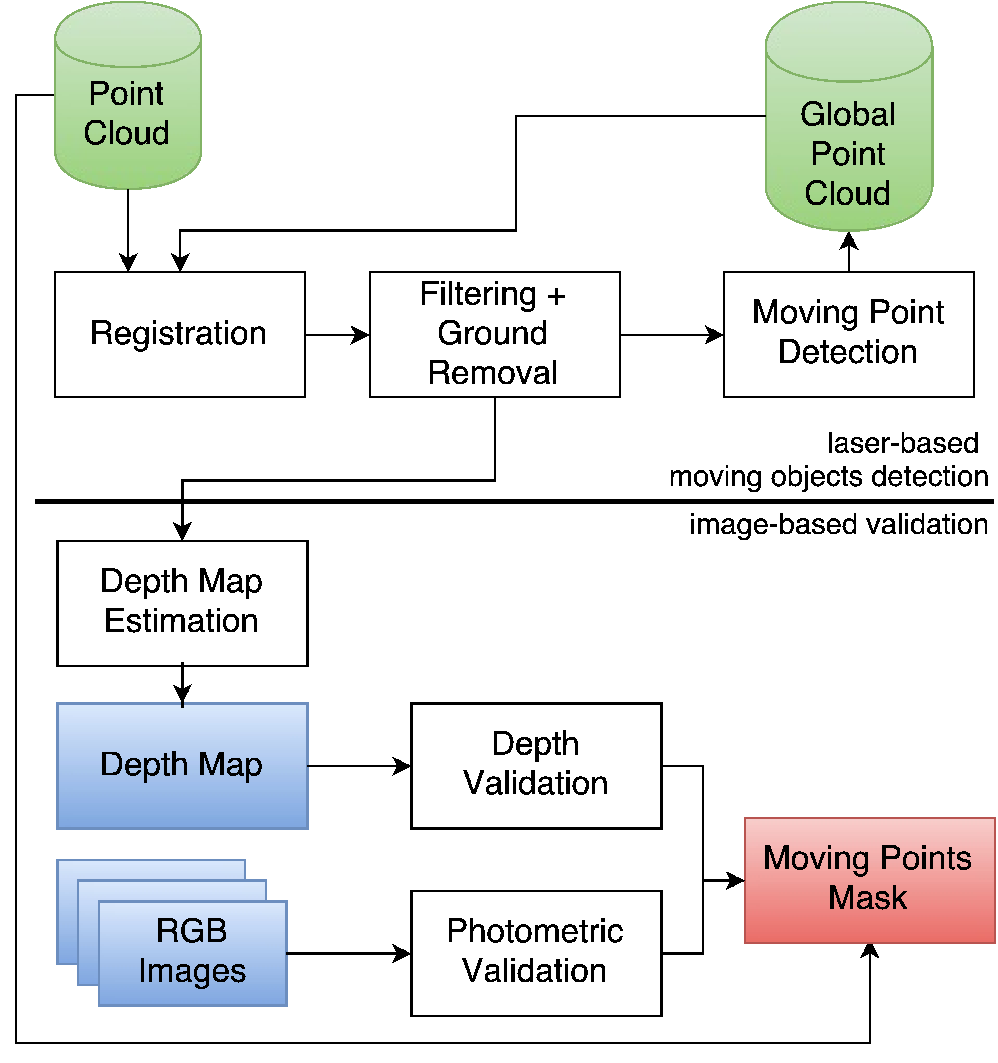
\includegraphics[width=0.98\columnwidth]{./img/ch-laser/MovingPointDetection}
\caption{Moving Object Detection process.}
\label{fig:algo}
\end{figure}
%
\subsection{Point cloud registration and filtering}
As a new point cloud is generated by the laser range finder, we align it to an existing map, initialized with the first scan, through the Generalized Iterative Closest Point (GICP) algorithm \cite{segal2009generalized}.
%
After point cloud alignment, we remove the points having a distance from the point cloud center greater than a given threshold $\tau = 30m$, along any of the three main axis to neglect points too faraway from the sensor.

Directly adding the aligned points to the map would lead to a very dense result, with possibly repeated points; instead, we compare the new point cloud with the last $W = 10$ 
point clouds we recently aggregated, and we add each point only if no other close point exist already in the map. This fills the gaps in point clouds and renders the global cloud free of duplicates\footnote{The use of the term duplicate, in this context, is improper since it is very unlikely the lidar samples exactly the very same point, but, assuming the sampling beam has non negligible size, we have overlapping regions sampled repeatedly and this would induce an unnecessary oversampling of the environment.}. Once the new points have been selected for addition, we further simplify the point cloud by ground plane removal.


\subsection{Ground plane removal}
\label{sec:ground_removal}
Subsequent laser measurements that lies on the ground plane convey redundant and negligible information about moving objects since the ground plane is expected to be mostly static. Therefore, as a further filtering step, we classify and remove ground plane points. 
A naive approach to do that would discard all points which are under a certain negative height from the laser sensor. 
A slightly better approach fits an horizontal plane, \eg, with RANSAC, and removes points which lay on it.
The drawback of both approaches arise whenever we deal with non-planar ground surface, as in Figure~\ref{fig:nonplane}, or errors in extrinsic sensor calibration.

\begin{figure}
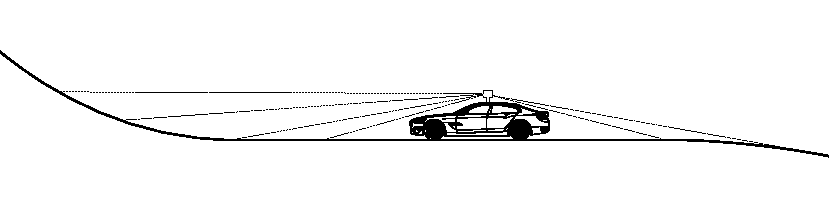
\includegraphics[width=0.99\columnwidth]{./img/ch-laser/./non-plane}
\caption{Non trivial example in which naive and plane fitting based ground removal fail.}
\label{fig:nonplane}
\end{figure}

\begin{figure}[t]
\centering
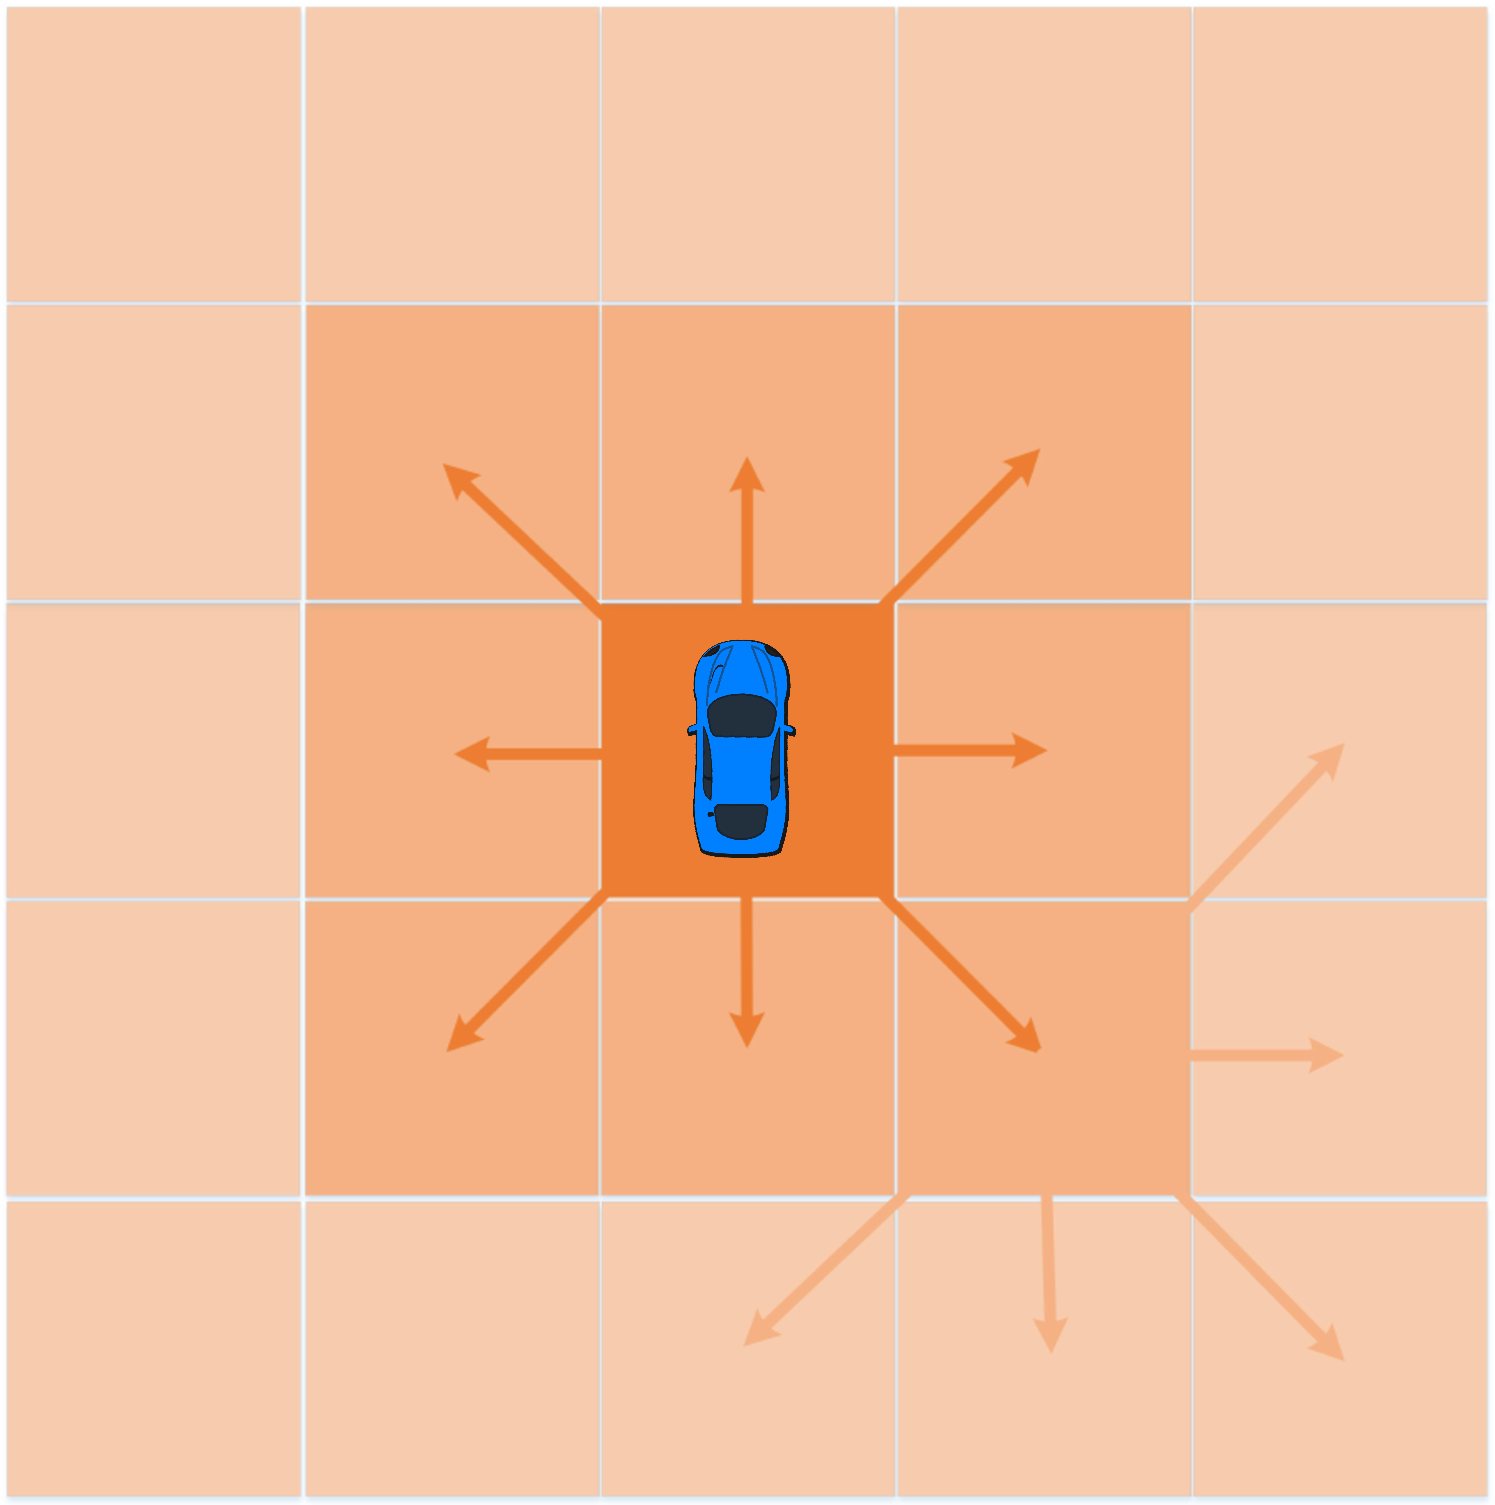
\includegraphics[width=0.99\columnwidth]{./img/ch-laser/groundpropagation}
\caption{Schema of ground height propagation.}
\label{fig:propag}
\end{figure}

We propose to remove the unnecessary ground points by modeling the ground as a Markov Random Fields and applying belief propagation as it follows. 
First, we divide the point cloud according to a 2D grid on the $XY$ plane, where $X$ represents the forward direction, and $Y$ points to the left side of the moving vehicle. 
Starting from the cell at the origin of this grid, supposedly being ground, we move iteratively to the surrounding cells in order to propagate the ground height and to classify the tiles between ground and non-ground (see Figure \ref{fig:propag}).
Let consider the cell $C_{ij}$ and the set $P_{ij}$ of the points projecting on this cell. We define $\hat{h}_G^{ij} = max\left\{h_G^N\right\}$ where $N$ is the set of neighboring cells, belonging to the inner ring, that propagate to  $C_{ij}$; then $H_{ij} = max{P_{ij}^z}$ and $h_{ij} = min{P_{ij}^z}$ are the maximum and minimum heights of the points in the cell (recall that coordinate $z$ represents the height of a point). 
Given a maximum expected slope of $22\%$ of the cell dimension, which is about $s=0.09m$; a cell is classified as ground plane if and only if:
\begin{equation}
H_{ij} - h_{ij} < s \qquad \text{and} \qquad H_{ij} < \hat{h}_G^{ij} + s.
\end{equation}
Then the current propagated ground height is:
\begin{equation}
   h_G^{ij} =  
      \begin{cases}
               H_{ij} \ \ & \text{if ${C}_{ij}$ is ground}\\
               \hat{h}_G^{ij} \ \ & \text{if ${C}_{ij}$ is non-ground}
        \end{cases}
\end{equation}

In Figure \ref{fig:groundremoval} we illustrate an example of the ground points detected in a single scan.



\begin{figure}
\setlength{\tabcolsep}{1pt}
\begin{center}
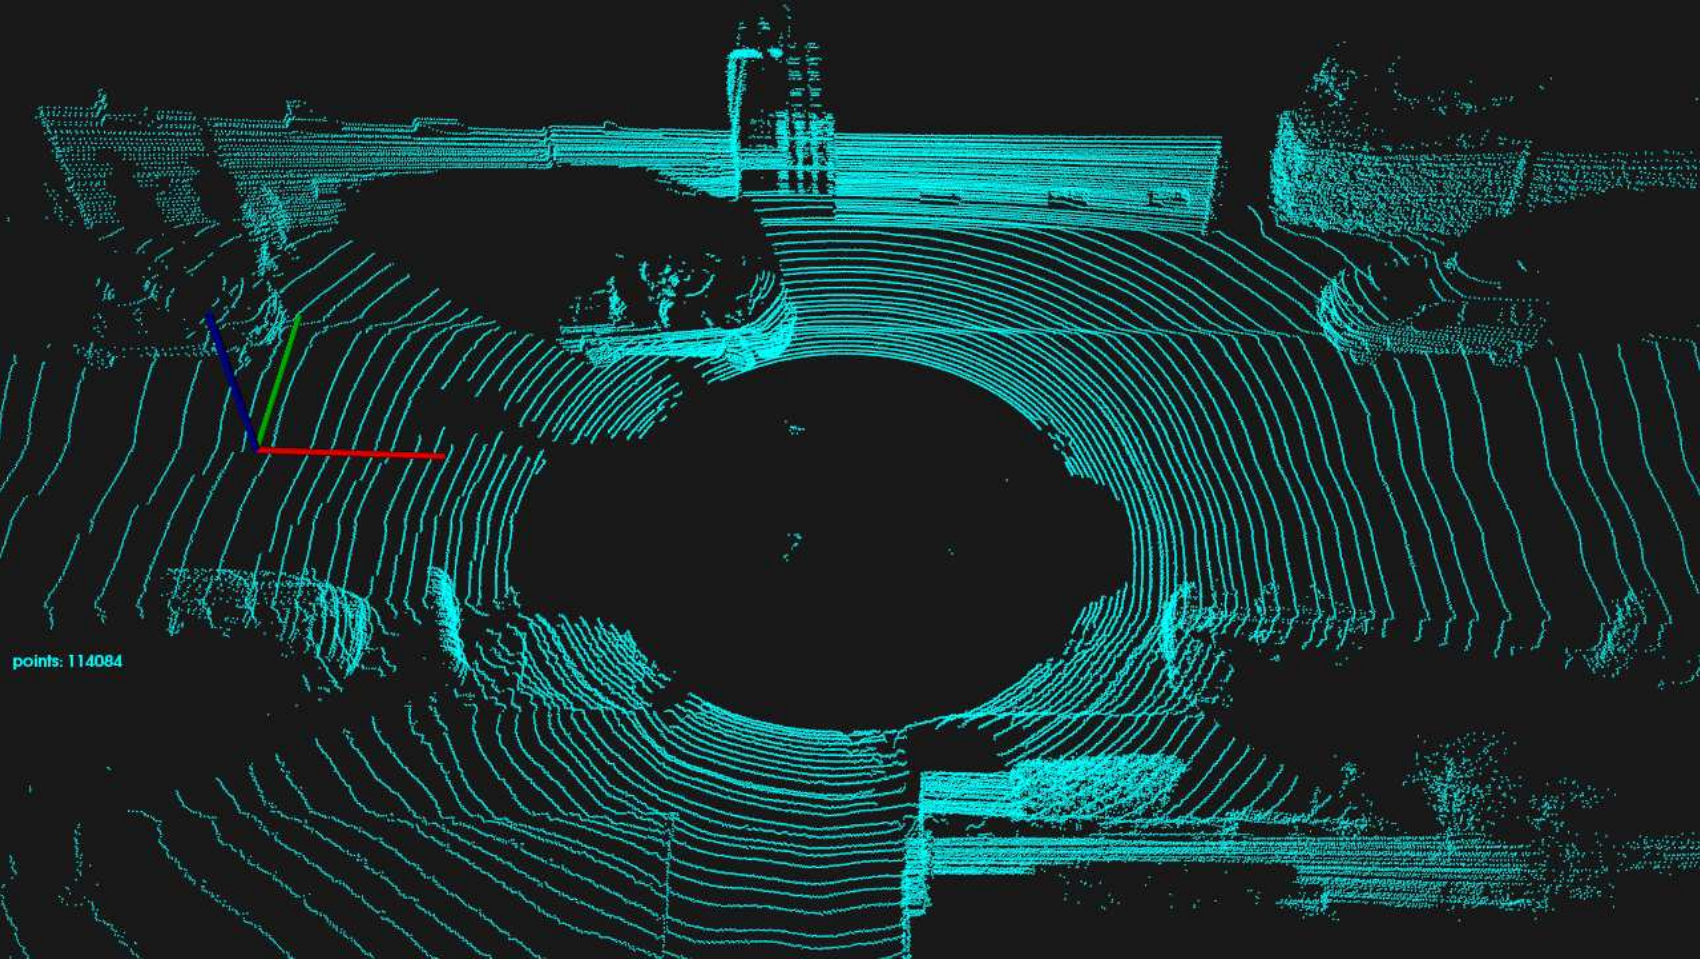
\includegraphics[width=0.99\columnwidth]{./img/ch-laser/beforeGroundRemoval} \\
\vspace{0.3cm}
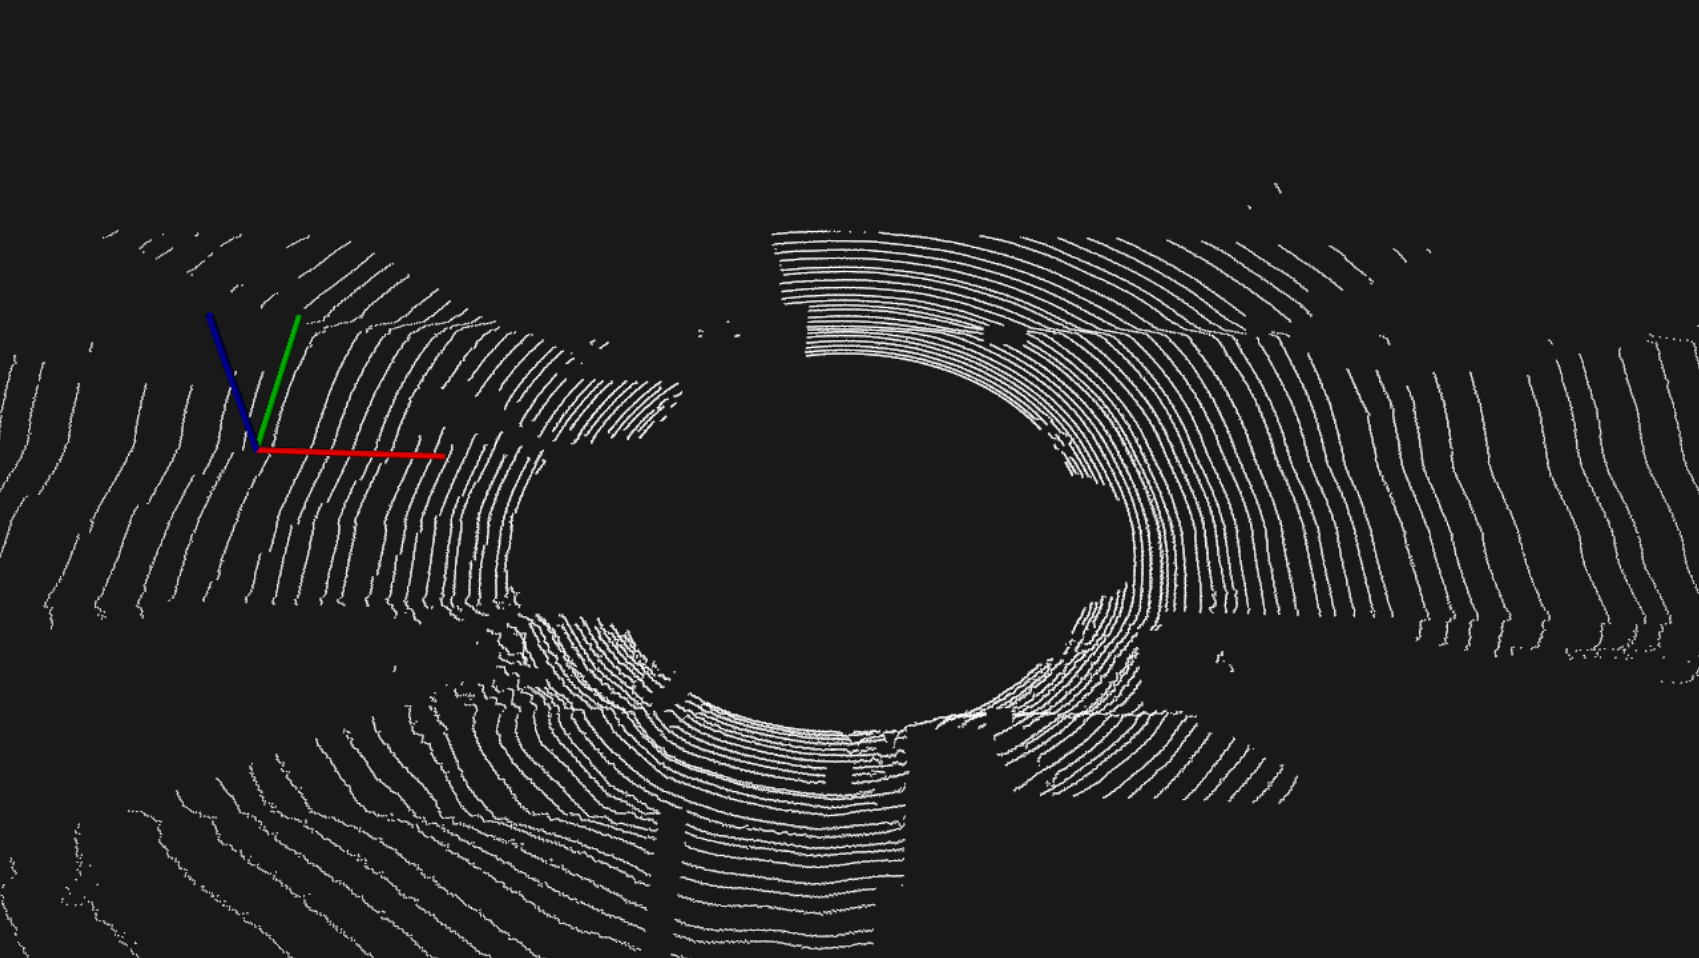
\includegraphics[width=0.99\columnwidth]{./img/ch-laser/postGroundRemoval}
\end{center}
\caption{A scan (above) and the ground points to be removed (below).}
\label{fig:groundremoval}
\end{figure}

\subsection{Moving Points detection}
After registration, point filtering, and ground removal we apply the laser-based moving object detection algorithm, which borrows some ideas from  \cite{xiao2013change} and \cite{vallet2015extracting}. From the former we borrow the use of Dempster-Shafer Theory (DST) for occupancy space representation and the Dempster-Shafer combination rule for intra-scan evidence fusion; from the latter we borrow the idea of using previous and future scans.
%\paragraph{Intra-Scan Fusion}

At first, we evaluate the occupancy of a point $P$ belonging to scan $S_{\text{k}}$ induced by another scan $S_{\text{i}}$ by representing the occupancy space using DST.  The space occupancy is represented using a set $X = \{empty, occupied\}$; the DST operates on the power set of $X$, \ie, $2^X = \{\{\emptyset\}, \{empty\}, \{occupied\}, \{empty,occupied\}\}$, where the subset $\{empty,occupied\}$ represents the $unknown$ state, \ie, the space not reached by the beams. DST defines a degree of belief $m(\cdot)$ for each subset: for the empty set it is 0 and for the other subsets they are within the range of $[0, 1]$ and they add up to a total of 1.

\begin{figure}[t]
\centering
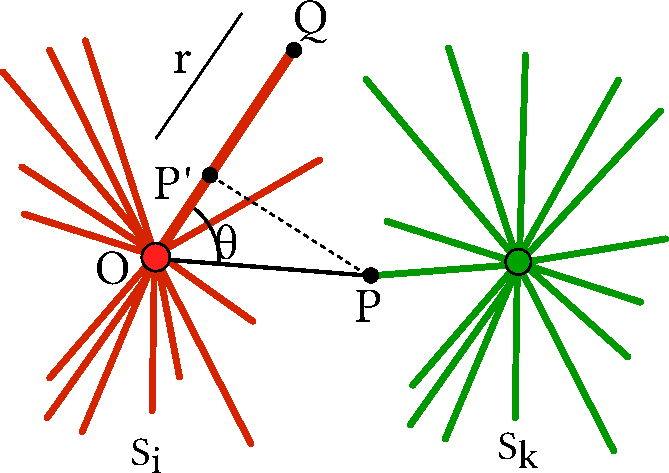
\includegraphics[width=0.99\columnwidth]{./img/ch-laser/scanoccupancy}
\caption{Occupancy at point $P$ computed with respect to the beam $OQ$.}
\label{fig:scanocc}
\end{figure}

Let  $e$~\shorteq~$m(\{empty\})$, $o$~\shorteq~$m(\{occupied\})$ and $u$~\shorteq~$m(\{unknown\})$ be the degrees of belief for the three possible labels such that $e + o + u$~\shorteq~$1$. 
Let $OQ$ be a laser beam of $S_i$, and $r$~\shorteq~$length(P'Q)$, where $P'$ is the projection of $P$ on $OQ$ (see Figure~\ref{fig:scanocc}); then we define the degree of belief $e_r$ and $o_r$ parametrized over $r$ as it follows:
\begin{align}
\label{eq:occ}
 e_r &=  \begin{cases}
               1 \ \ & \text{if $Q$ is behind $P'$}\\
               0 \ \ & \text{otherwise}
         \end{cases},\\
\label{eq:occ_2}
o_r &=  \begin{cases}
      e^{-\frac{r^2}{2}} \ \ & \text{if $P'$ is behind $Q$}\\
      0 \ \ & \text{otherwise}
        \end{cases}.
\end{align}
The occupancy values at point $P$ due to the beam $OQ$ becomes then:
\begin{equation}
\label{eq:comb}
 m(P,Q)=\left\{\  \begin{aligned}
                 e\\o\\u
                 \end{aligned}
\  \right\} = \left\{\  \begin{aligned}
                     f_\theta&\cdot e_r \ \\
                     &o_r \ \\
                     1 - &e - o \ 
                    \end{aligned}
\ \right\}\\
\end{equation}
where $f_\theta = e^{-\frac{\theta^2}{2\lambda_\theta^2}}$ is the rotation occupancy function, $\lambda_\theta$ is the angular resolution of the sensor, and $\theta$ is the angle between rays $OP$ and $OQ$.


To embed uncertainty in this framework, we propose to model noise as a Gaussian variable, then we define $\sigma_m$, $\sigma_r$ and $\sigma_\theta$ as, respectively, measurement, registration, and angle standard deviations (with $\sigma_m=0.05$, $\sigma_r=0.15$, $\sigma_{\theta}=0.1\pi$). 
By defining  $g(m) = \mathcal{N}(0, \sigma_m^2)$, $g(r) = \mathcal{N}(0, \sigma_r^2)$, $F = g(m)\otimes g(r)$, we modify \eqref{eq:comb} as it follows:

\begin{equation}
 m'(P,Q)=\left\{\  \begin{aligned}
                 e'\\o'\\u'
                 \end{aligned}
\  \right\} = \left\{\  \begin{aligned}
                     f_\theta  &\cdot (e_r \otimes F)\\
                     &o_r \otimes F\\
                     1 - &e' - o'\\ 
                    \end{aligned}
\ \right\}
\end{equation}
where $\otimes$ represents the convolution operator.
We  aggregate the occupancy induced by two beams through the Dempster-Shafer combination rule applied to the occupancy induced by two beams with $m(P,Q_1)=(e_1, o_1, u_1)$ and $m(P,Q_2)=(e_2, o_2, u_2)$:

\begin{equation}
%\scriptsize
  \left\{ \begin{aligned}
                 e_1\  \\o_1\  \\u_1\ 
                \end{aligned}
 \right\} \oplus \left\{ \begin{aligned}
                     e_2\ \\o_2\ \\u_2\  
                    \end{aligned}
\right\} = \frac{1}{1-K} 
\left\{ 
  \begin{aligned}
     &e_1\cdot e_2 + e_1\cdot u_2 + u_1\cdot e_2 \ \\
     &o_1\cdot o_2 + o_1\cdot u_2 + u_1\cdot o_2 \ \\
     &u_1\cdot u_2 \ 
  \end{aligned}
 \right\}
\end{equation}
where $\oplus$ is the fusion operator defined by DST which is commutative and associative, and $K = o_1\cdot e_2 + e_1\cdot o_2$.
From this, the overall occupancy at location $P$ due to the $I$ neighboring rays $Q_i$ is then given by:
\begin{equation}
 m(P) = \bigoplus_{i\in I} m(P,Q_i).
\end{equation}

%\paragraph{Inter-Scan Consistency}
To classify a point $P$ belonging to a scan $S_{\text{k}}$ as static or moving, we compute and combine its occupancy values due to previous and future\footnote{We observe a time window of $2K$ scans around the current one, with $K=10$ in our experiments, introducing a K scans delay in the whole pipeline.} scans $\mathbb{S} = \{S_{\text{k-K}}, \dots, S_{\text{k-1}}, S_{\text{k+1}}, \dots, S_{\text{k+K}} \}$.
By comparing two scans having the degree of belief $m(P,Q_1)$ and $m(P,Q_2)$, a moving object corresponds to the not consistent degree of belief. To this extent, we compute:
\begin{equation}
 \begin{split}
  Conf &= e_1\cdot o_2 + o_1\cdot e_2\ \\
  Cons &= e_1\cdot e_2 + o_1\cdot o_2 + u_1\cdot u_2\ \\
  Unc\ &= u_1\cdot (e_2 + o_2) + u_2\cdot (e_1 + o_1)\\
 \end{split}
\end{equation}
where $Conf$ means conflicting, $Cons$ is consistent and $Unc$ uncertain. 
Moving points regions are those where $Conf > Cons$ and $Conf > Unc$. 
We have extended this procedure, originally proposed in \cite{xiao2013change} for 2 scans, to compare $2K$ subsequent scans.
%\paragraph{Discretizing the Occupancy}
To do so, we propose to change the occupancy computation procedure in order to make the classification more robust by a novel discretized version of the original approach we just explained. 

Let consider the most distant point $B$ in each scan $S_{\text{i}} \in \mathbb{S}$, we approximate the occupancy values of $P$ with respect to $S_{\text{i}}$ in the following way. Let's define 
\[
 l = r_{sup} - \delta r\frac{||\overrightarrow{OP}||}{||\overrightarrow{OB}||}
\] 
where $r_{sup}$ and $r_{inf}$ are user defined upper and lower bounds and $\delta r = r_{sup} - r_{inf}$ (in our case  $r_{sup} = 0.8$ and $r_{inf} = 0.6$); $l$ is used to define a belief stronger in the neighborhood of the sensor. Then, from the original occupancy $m(P,Q)=(e, o, u)$ we derive the new occupancy of $P$ for any $Q\in S_{\text{i}}$:
\begin{equation}
 e_{\text{new}} = \begin{cases}
      l\ \ \ &\mbox{if }e > o \wedge e > u \\
      0 &\mbox{otherwise}
     \end{cases}
\end{equation}

\begin{equation}
 o_{\text{new}} = \begin{cases}
      l\ \ \ &\mbox{if }o > e \wedge o > u \\
      0 &\mbox{otherwise}
     \end{cases}
\end{equation}

\begin{equation}
 u_{\text{new}} = 1 - e_{\text{new}} - o_{\text{new}}.
\end{equation}

 This way the occupancy value of each point is discretized based on its distance from the sample scan origin. With these discretized values we apply again the Dempster-Shafer combination rule among the set $\mathbb{S}$ of scans, and the outcome of this combination defines the classification of the point: if its prevalent occupancy state is $empty$ then the point is considered to be dynamic, otherwise it is a static point. 
  
%We impose the default occupancy state of a point to $unknown$ if this point is outside the bounding box of the other scan. If the point is inside the bounding box, but it has no neighbors, it is more likely to be a non-stationary point, and for this reason it is given a predefined state, weighted more towards $empty$. The ground points are removed only from the scan $S_{\text{k}}$, and are kept in the scans in $\mathbb{S}$. This is done first to avoid testing the ground points (as they are assumed to be always static), and second it allows to have neighboring rays which hit the ground in sample scans and thus identify potential dynamic points. Once the dynamic points are identified, they are removed from scan $S_{\text{k}}$ and they are kept in a data structure for future use. 
 
%\subsection{Efficient octree implementation}%%%%%%%%%
% In the proposed approach, we transform the points of each scan are into spherical coordinate system then they are indexed by a Kd-tree data structure using only the two angles $\theta$ and $\phi$. This allows a fast neighborhood search for points and thus significantly reduces the computational time.

Testing every point $P$ from a scan $S_{\text{k}}$ against every neighboring ray in the $\mathbb{S}$ scans is a very expensive procedure. 
We avoid such expensive computations by indexing the $S_{\text{k}}$ point cloud with an octree data structure, with a resolution of 0.3m, and we perform the tests only for a small set of points in its nodes, \ie, in the neighborhood of the point $P$.
Since dynamic points in real world are not sparse, as they are part of a moving object, we assume they have neighboring dynamic points, and, if a small set of neighboring points are classified as dynamic, their neighbors should also be considered dynamic as well. 
Thus, to improve the performance of our algorithm, for each leaf of the octree, we perform the moving object detection test on a random subset of points ($\frac{1}{6}$ of the total amount) and if there are at least half of the tested points classified as dynamic, then we classify all the points in the leaf as such. Otherwise, the leaf is assumed to contain only static points.
If the number of points in a leaf is small, \ie, less than $\tau_{np}=6$, they are sparse and they all get tested. By doing this way, we do not only improve the computational efficiency of the algorithm, but we also reduces the amount of misclassified dynamic points in static objects.


\section{Image-based Moving Object Validation}%%%%%%%%%%%%%%%%%%%%%%%%%%%%%%%%%%%%%%%%%%%%%%%%%%%%%%%%%%
\label{sec:images}
Even if the outcome of our laser-based moving object detection algorithm is often satisfying, some false positives may arise due to the noise in the laser measurements and the inaccuracy of the point cloud registration step. 
We propose thus two additional image-based validation tests to filter out false positives: both tests compare image patches around the projection of 3D points classified as moving objects respectively in the (color) images corresponding to the scans in $\mathbb{S}$ and in the depth-maps estimated from the point clouds themselves. If a candidate point passes these tests, then it is confirmed to be a moving point.

In the proposed tests a 3D point $P_i$ is projected into a pixel $p_{ik}$ of the (color) image $I_k$ and depth map $D_k$ by using the camera calibration matrix. A squared image patch $patch_{ik}$ around this pixel is selected having a side length $b_{ik}$, measured in number of pixels, according to the following formula:
\begin{equation}
 b_{ik} = \frac{h}{d_{ik}}f_{xy},
\end{equation}
where the $h=0.15m$ parameter refers to the patch height in the real world, $d_{ik}$ is the distance of the point $P_i$ from the camera $k$ corresponding to pixel $p_{ik},$ and $f_{xy}$ is the focal length of the camera (see Figure \ref{fig:ncc}).
Since each comparison needs two patches of the same size, one of the two patches, in turn, is resized.

Before computing any similarity between images patches, these are checked for uniformity in their intensities. If their intensity standard deviation is above a certain threshold, then we compare the color patches, otherwise, the test would fail, so we compare directly the depth maps.

\subsection{Image patch test}%%%%%%%%%%%%%%%%%%%%%%%%%%%%%%%%%%%%%%%%%%%%%
Once patches are extracted and resized, we test their similarity through Normalized Cross Correlation (NCC) on each color channel independently. 
Let $\pi_i$ and $\pi_j$ be the two patches and $NCC_c(u,v)$ the NCC between two images at location $(u,v)$ computed for the $c$-th channel, then we define:
\begin{equation}
 E_k(\pi_i, \pi_j) = 1 - \max_{u,v}NCC_k(u,v).
\end{equation}
Two patches are considered to be similar if, for all cameras in $\mathbb{S}$, $E_k < \tau$ (in our case $\tau=0.1$). 

We opted for NCC measure with respect to the other classical Sum of Squared Differences(SSD), since it is not affected by illumination changes issue, even thought it is computationally more expensive than SSD. Note that, if one of the patches has one of its channels flat, the formula above fails, as we get a division by zero problem for the NCC computation. Our system handles this case with the second test on the depth-maps. 

\subsection{Depth-map patch test}%%%%%%%%%%%%%%%%%%%%%%%%%%%%%%%%%%%%%%%%%%%%
When the color image patch test fails, we apply a comparison between the depth-maps extracted from the lidar data as it follows.
We project lidar points into the $k$-th camera, by using the camera matrix, and we create a sparse depth-map having for each pixel the camera-to-point distance. Then we apply a disk shaped dilation such that we close all the gaps between close points.
The resulting image is a rough estimation of the depth-map of the lidar points, nevertheless its computation is fast and the result has been sufficiently discriminative in our tests (Figure \ref{fig:depth-map} shows an example of a depth-map extracted from the laser data).


\begin{figure}[t]
\centering
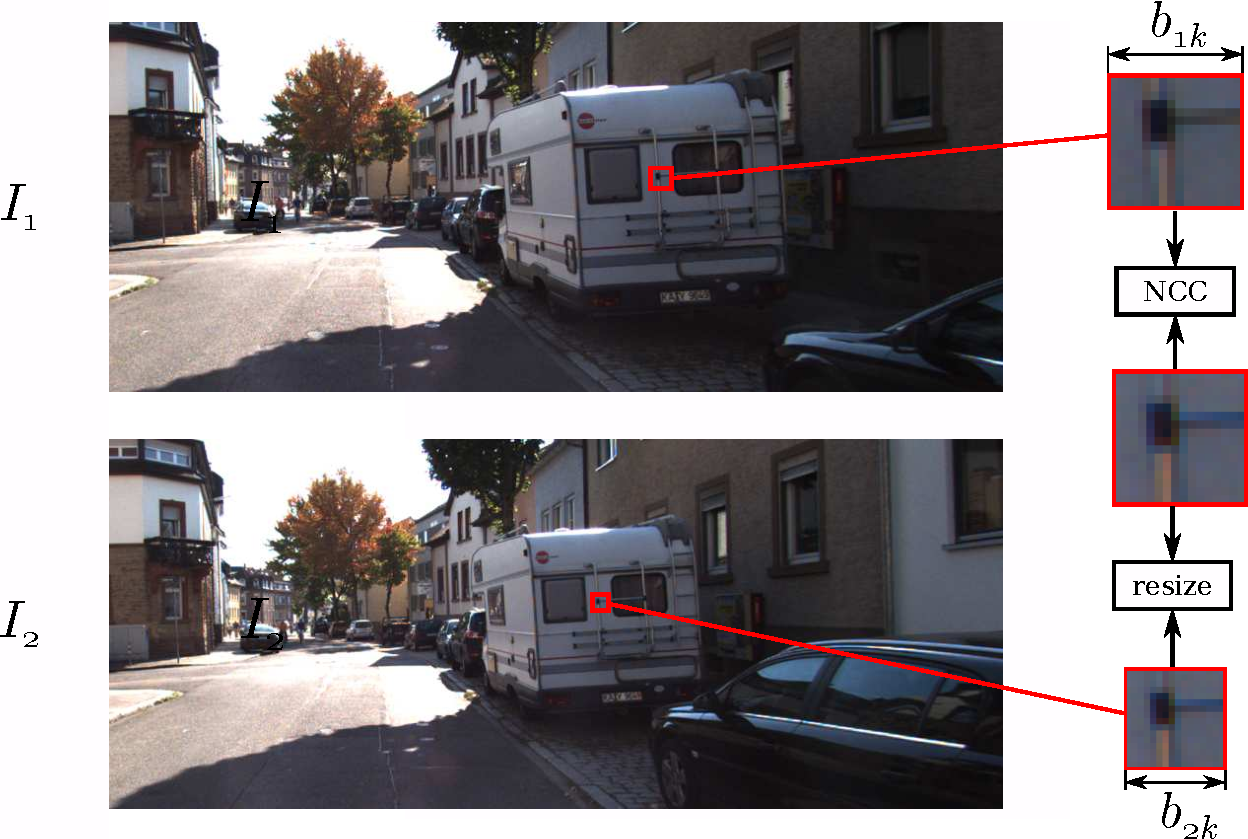
\includegraphics[width=0.98\columnwidth]{./img/ch-laser/ncc}
\caption{Example of two color patches compared via NCC.}
\label{fig:ncc}
\end{figure}

Since the laser sensor is moving between the two scans, we need to correct the depthmaps for this movement before we can actually compare the selected patches.
%before patch comparisons on the so computed depth maps, the images should have comparable intensities. 
To perform this correction, we assume a small motion between two cameras and we use the following formula:
\begin{equation}
D_l' = D_l + \frac{||\mathbf{t}_k - \mathbf{t}_l||}{d_{l,max}}
\end{equation}
where $D_l'$ and $D_l$ are respectively the new and old intensity values of depth map $l$, $\mathbf{t}_k$ and $\mathbf{t}_l$ are translation vectors, with respect to a global reference frame, for cameras $k$ and $l$ respectively, and $d_{l,max}$ is the maximum depth distance from the camera $l$.

\begin{figure}[t]
\centering
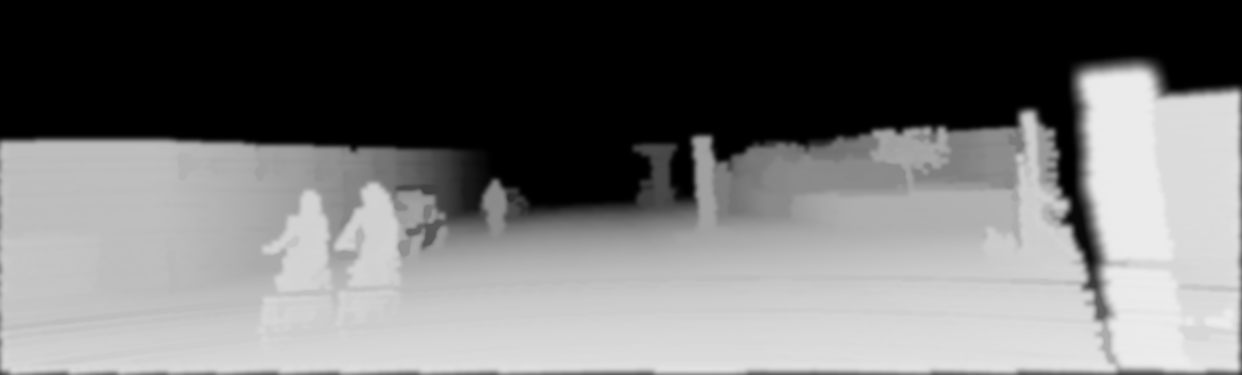
\includegraphics[width=0.98\columnwidth]{./img/ch-laser/depth-0129}
\caption{Example of a depthmap computed from a lidar point cloud.}
\label{fig:depth-map}
\end{figure}

Then patches are extracted and resized the same way we do for (color) images, but in the depthmap comparison we use the SSD metric. This metric is suitable in this case because depthmaps are not affected by illumination changes.



\section{Textured Mapping without moving objects}
Once the moving object have been removed, we build a map of the environment by relying on the methods presented in the previous chapters.
In particular we aim at reconstructing a texturized map of the environment, where moving objects are deleted, therefore not just a plain image projection on the surface mesh such as \ref{fig:recwithoutmoving}.



\begin{figure}[tp]
 \centering
    \begin{tabular}{c}
    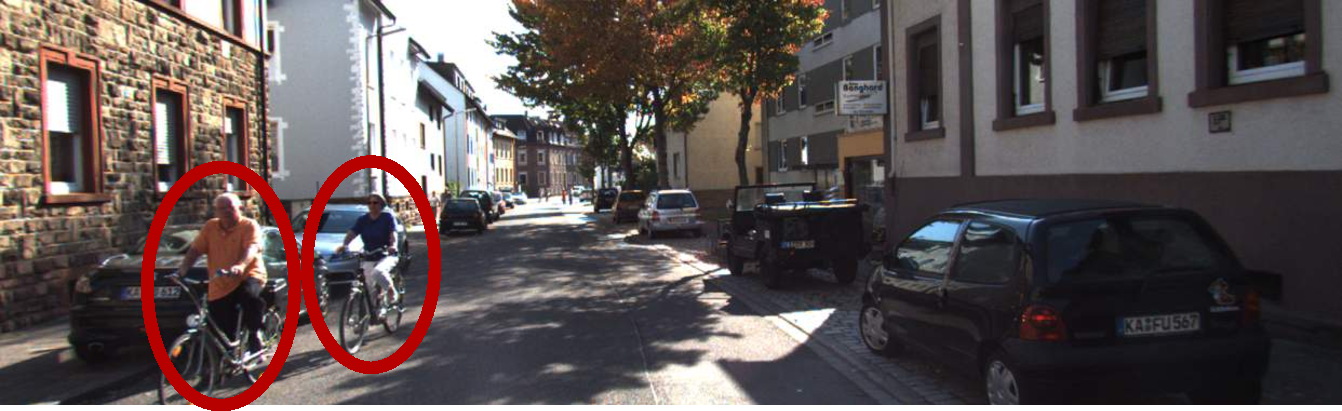
\includegraphics[width=0.92\columnwidth]{./img/ch-laser/originaFrame}\\
    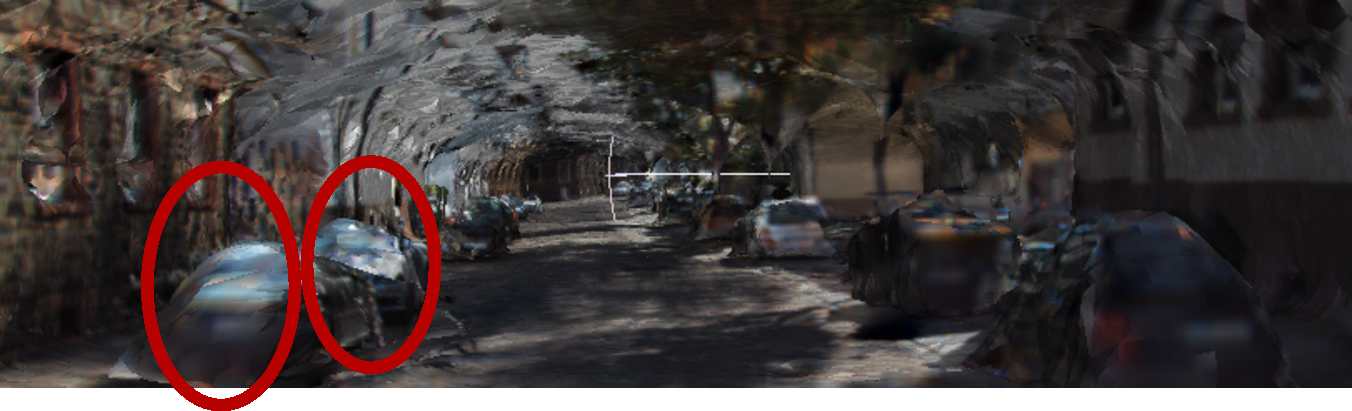
\includegraphics[width=0.92\columnwidth]{./img/ch-laser/texuredRec}\\
 \end{tabular}
 \caption{Textured mesh reconstructed from the KITTI sequence. Notice how moving objects do not appear in the final results}
 \label{fig:recwithoutmoving}
\end{figure}



\subsection{Laser-based 3D mapping}
The previous steps output a downsampled lidar point cloud without the moving objects, and the positions of the laser range finder in metric coordinates after the GICP registration.
We also know the visibility rays that goes from each laser scan to the perceived 3D points. These data perfectly fits in the visibility-consistent reconstruction algorithm presented in Chapter \ref{ch:manif}.

%; moreover, the algorithm ensure the manifold property of the mesh which is needed for the photometric refinement.
However, in real applications, we deal with glass or transparent surfaces, \eg, the windows of cars and houses; the laser beams traverse those surfaces, opposed to image-based reconstruction adopted in Chapter \ref{ch:manif}, which, even if it provides less accurate 3D estimation, it neglects natively these points.
Therefore, laser-based reconstruction is not able to capture adequately the geometry of the scene in the presence of transparent surfaces. 
In the particular case of car windows, the rays traverse the interior of the car from different points of view, and, the visibility consistent reconstruction would carve almost all the space occupied by the car, leaving only its lower part in the reconstruction.
To avoid this undesired behavior, we propose to detect the cars in the point cloud and replace their points with a 3D model of it, \eg, Fig. \ref{fig:cardetection2}.

\begin{figure}[tp]
 \centering
    \begin{tabular}{cc}
    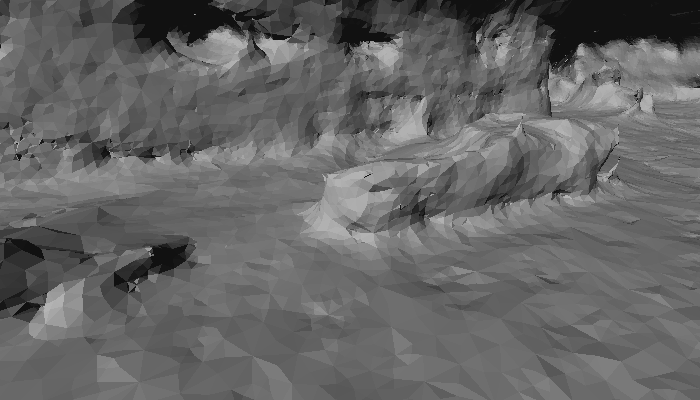
\includegraphics[width=0.4\columnwidth]{./img/ch-laser/base00_}&
    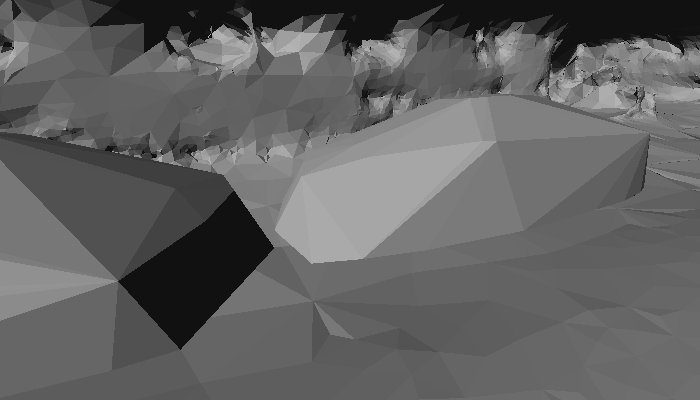
\includegraphics[width=0.4\columnwidth]{./img/ch-laser/car00_}\\
    (a)&
    (b)\\
    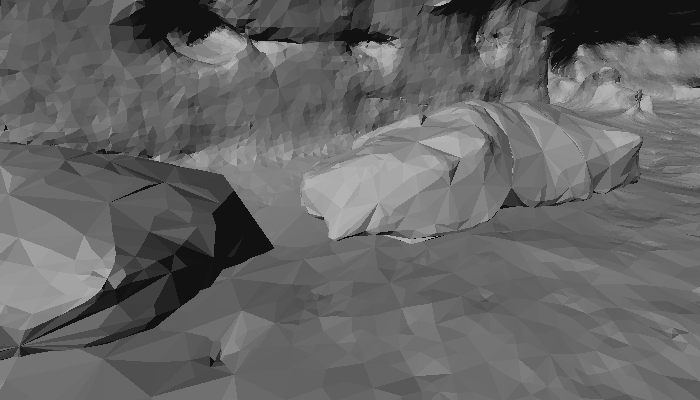
\includegraphics[width=0.4\columnwidth]{./img/ch-laser/nottext00_}&
    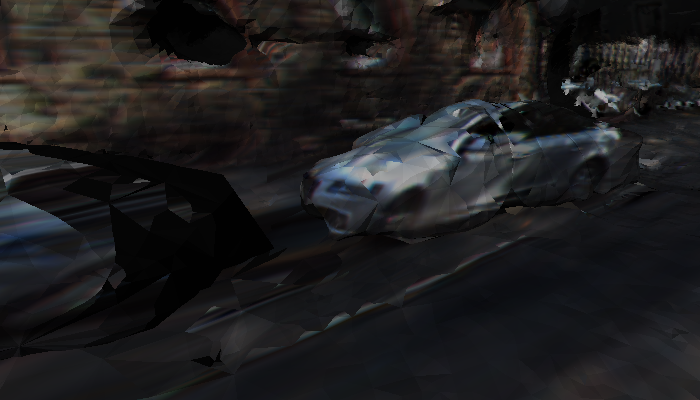
\includegraphics[width=0.4\columnwidth]{./img/ch-laser/text00_}\\
    (c)&
    (d)
 \end{tabular}
 \caption{Reconstruction of Lidar data: (a) with the visibility consistency \cite{romanoni15b}; (b) with the proposed car detection; (c) with the proposed car detection and refinement and (d) after texturing}
 \label{fig:cardetection2}
\end{figure}






\begin{figure}[tp]
 \centering
    \begin{tabular}{c}
    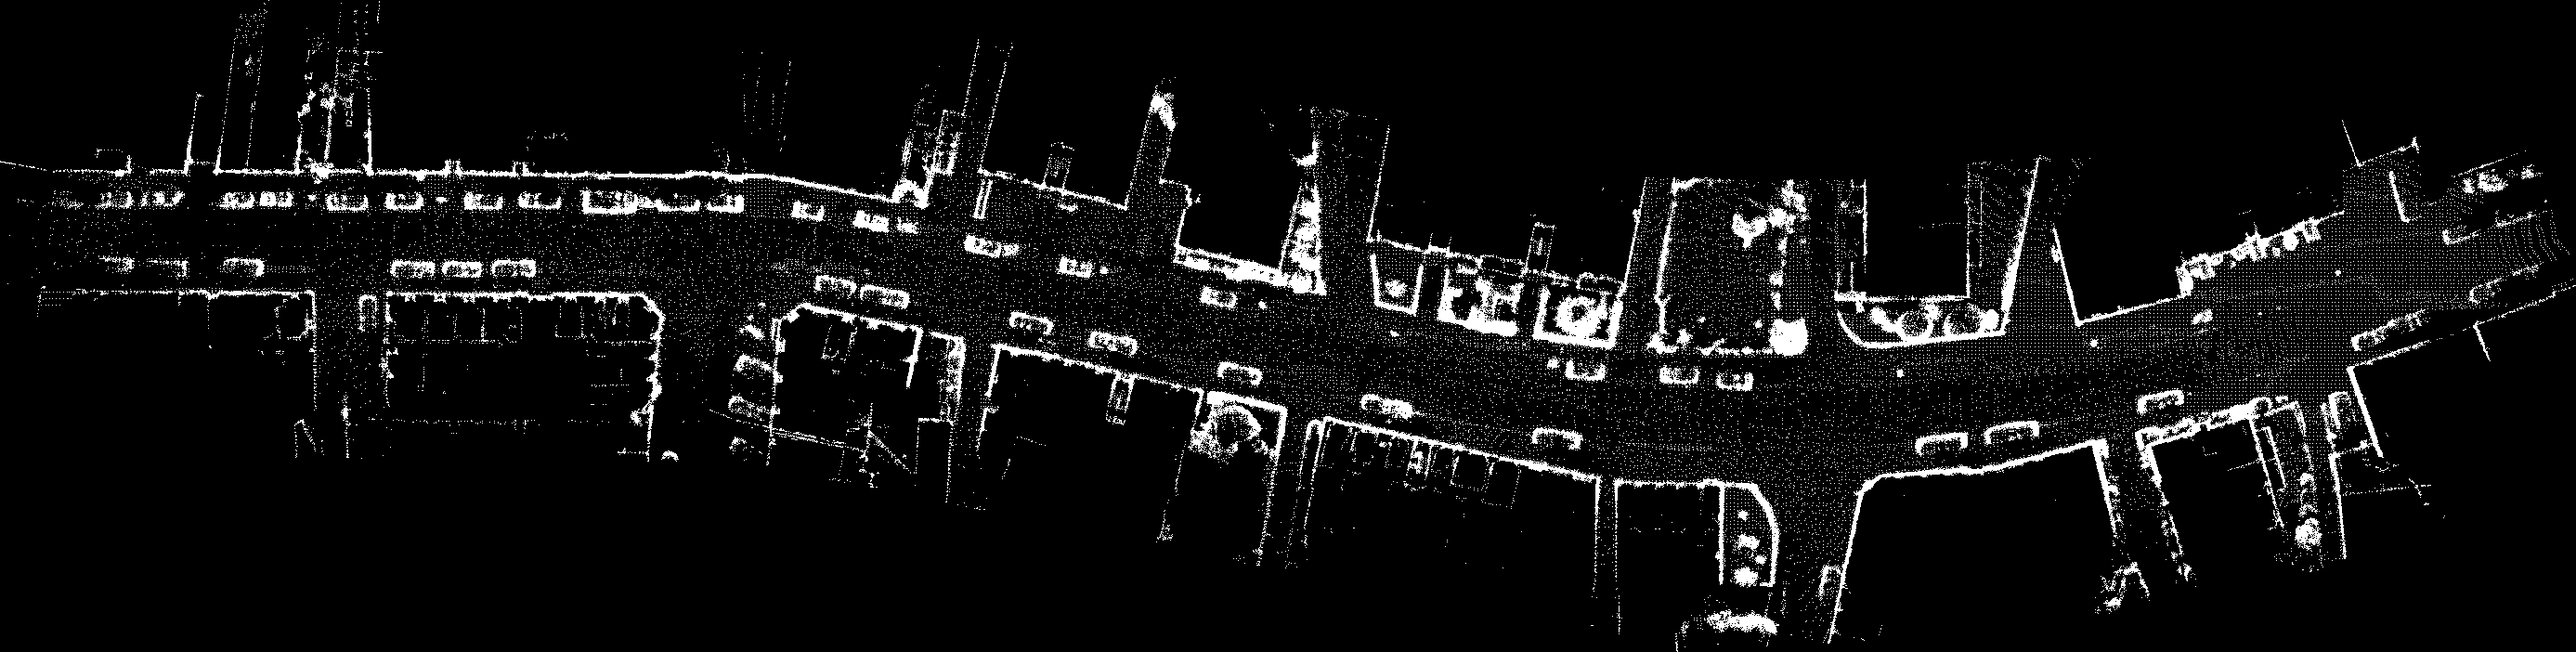
\includegraphics[width=0.92\columnwidth]{./img/ch-laser/pointsprojected}\\
    (a)\\
  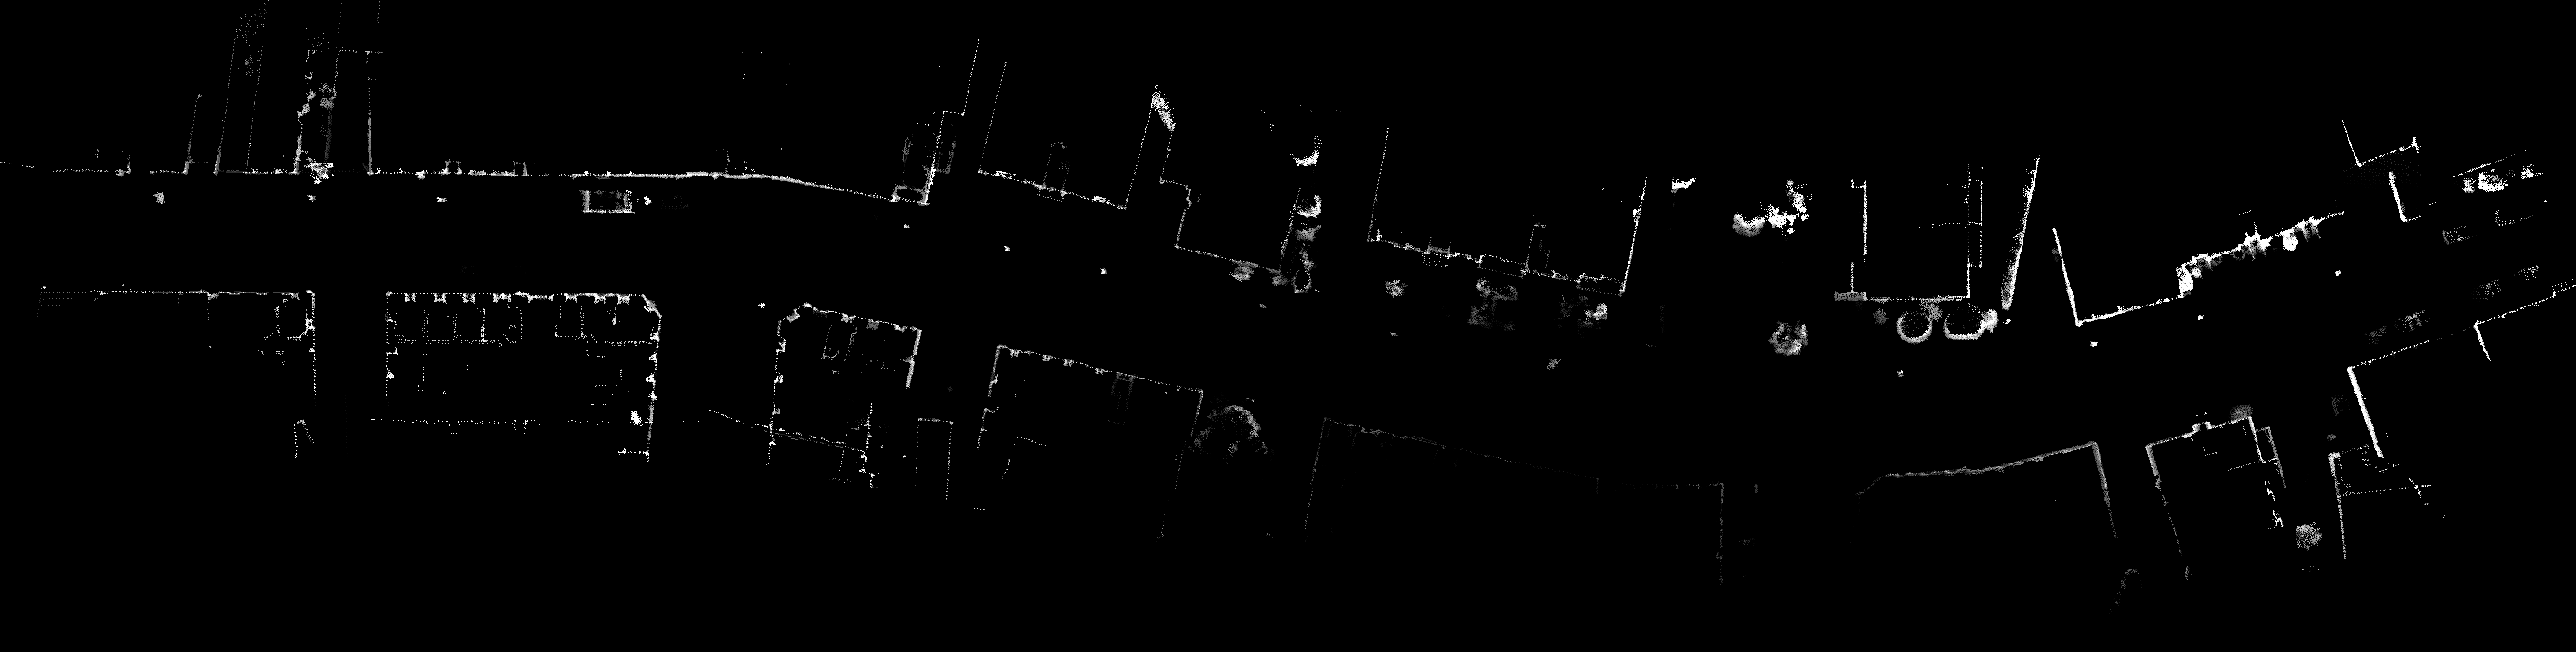
\includegraphics[width=0.92\columnwidth]{./img/ch-laser/heightimagePointsProjected_.png}\\
    (b)\\
  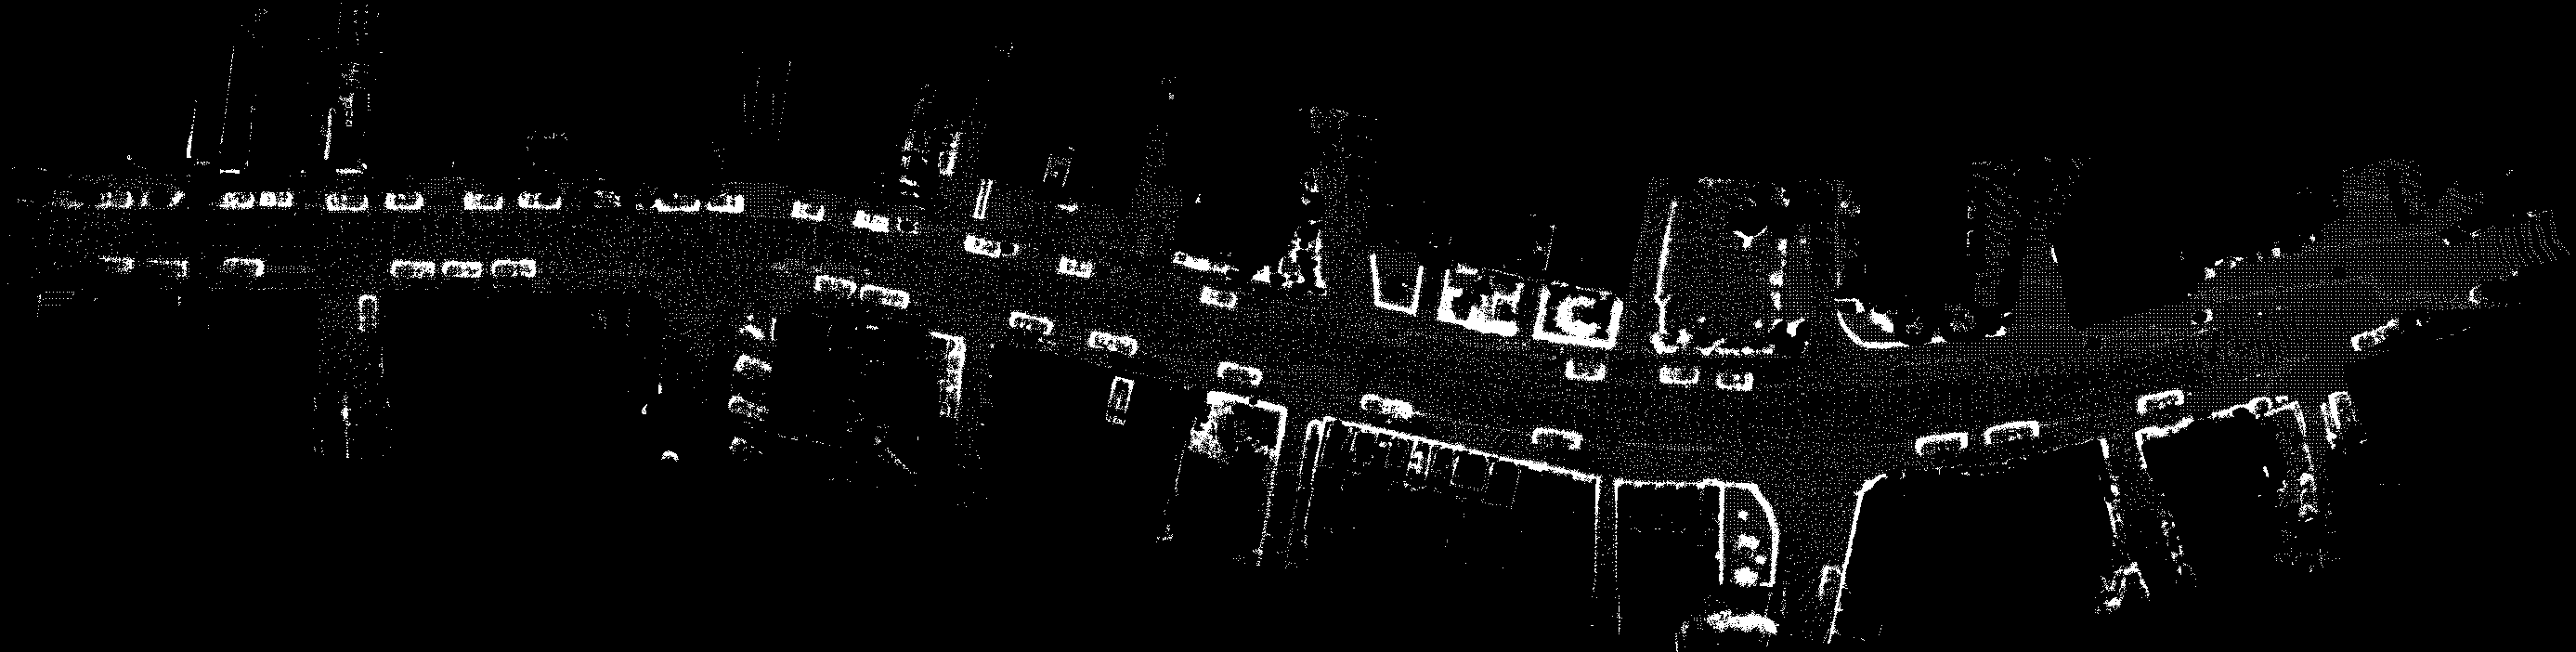
\includegraphics[width=0.92\columnwidth]{./img/ch-laser/pointsprojectedFiltered.png}\\
    (b)\\
  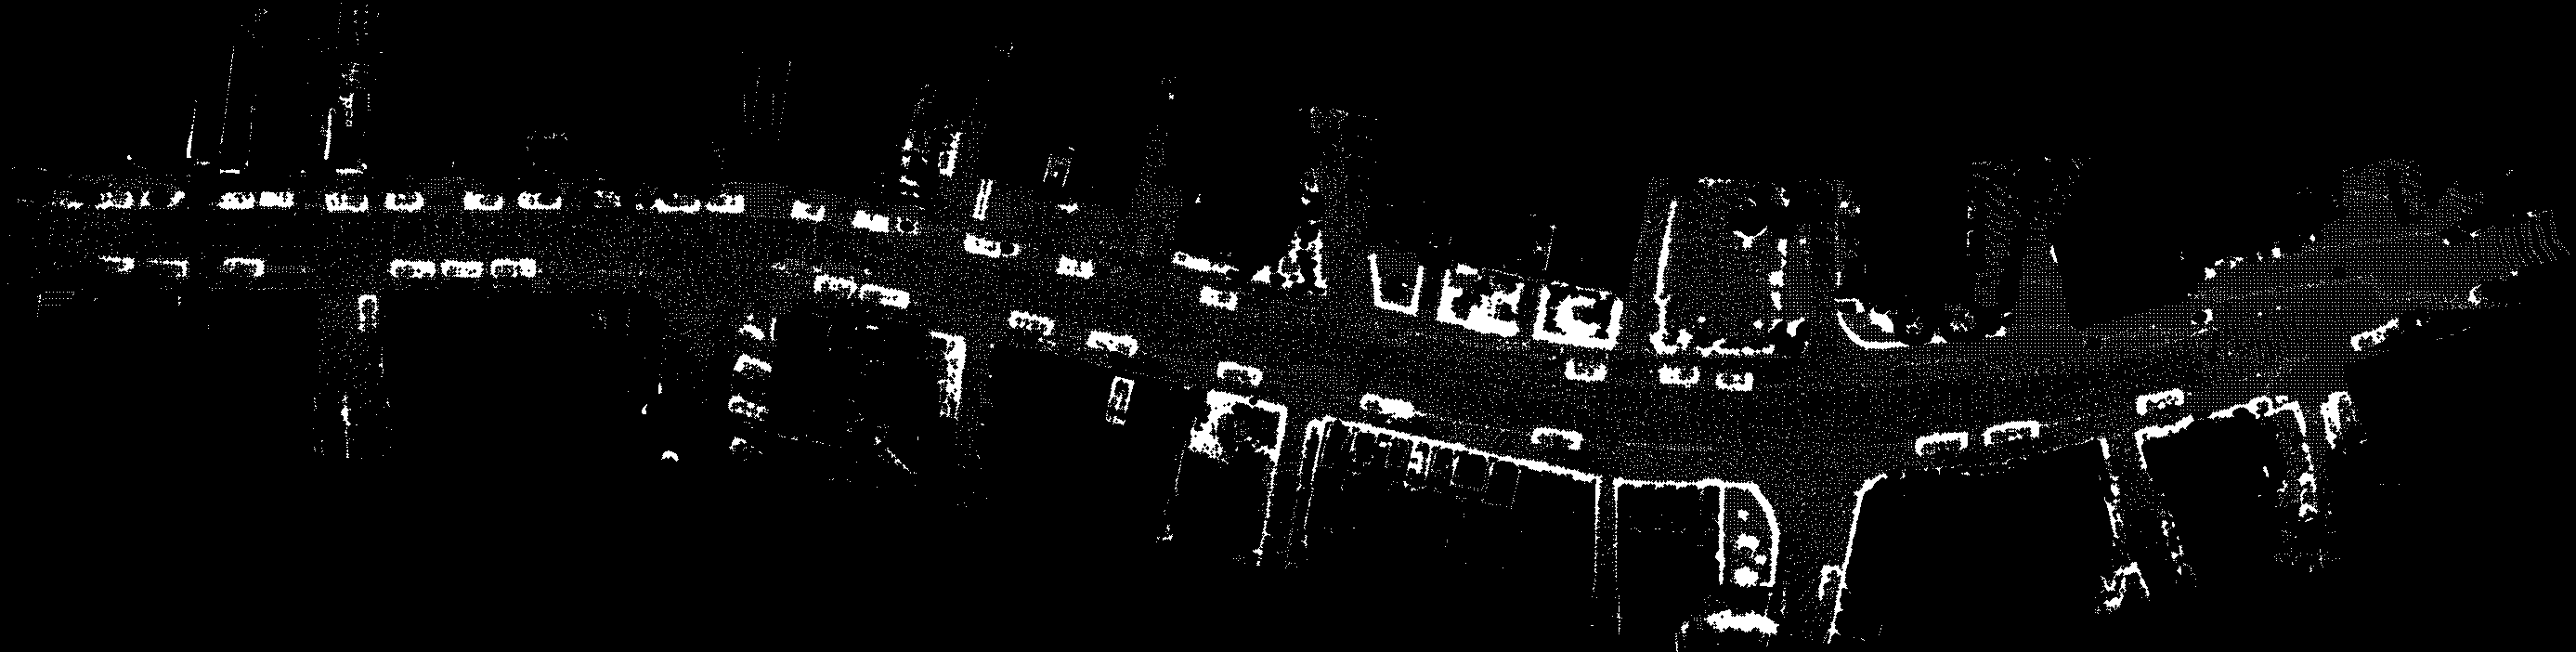
\includegraphics[width=0.92\columnwidth]{./img/ch-laser/pointsprojectedEroded.png}\\
    (b)\\
    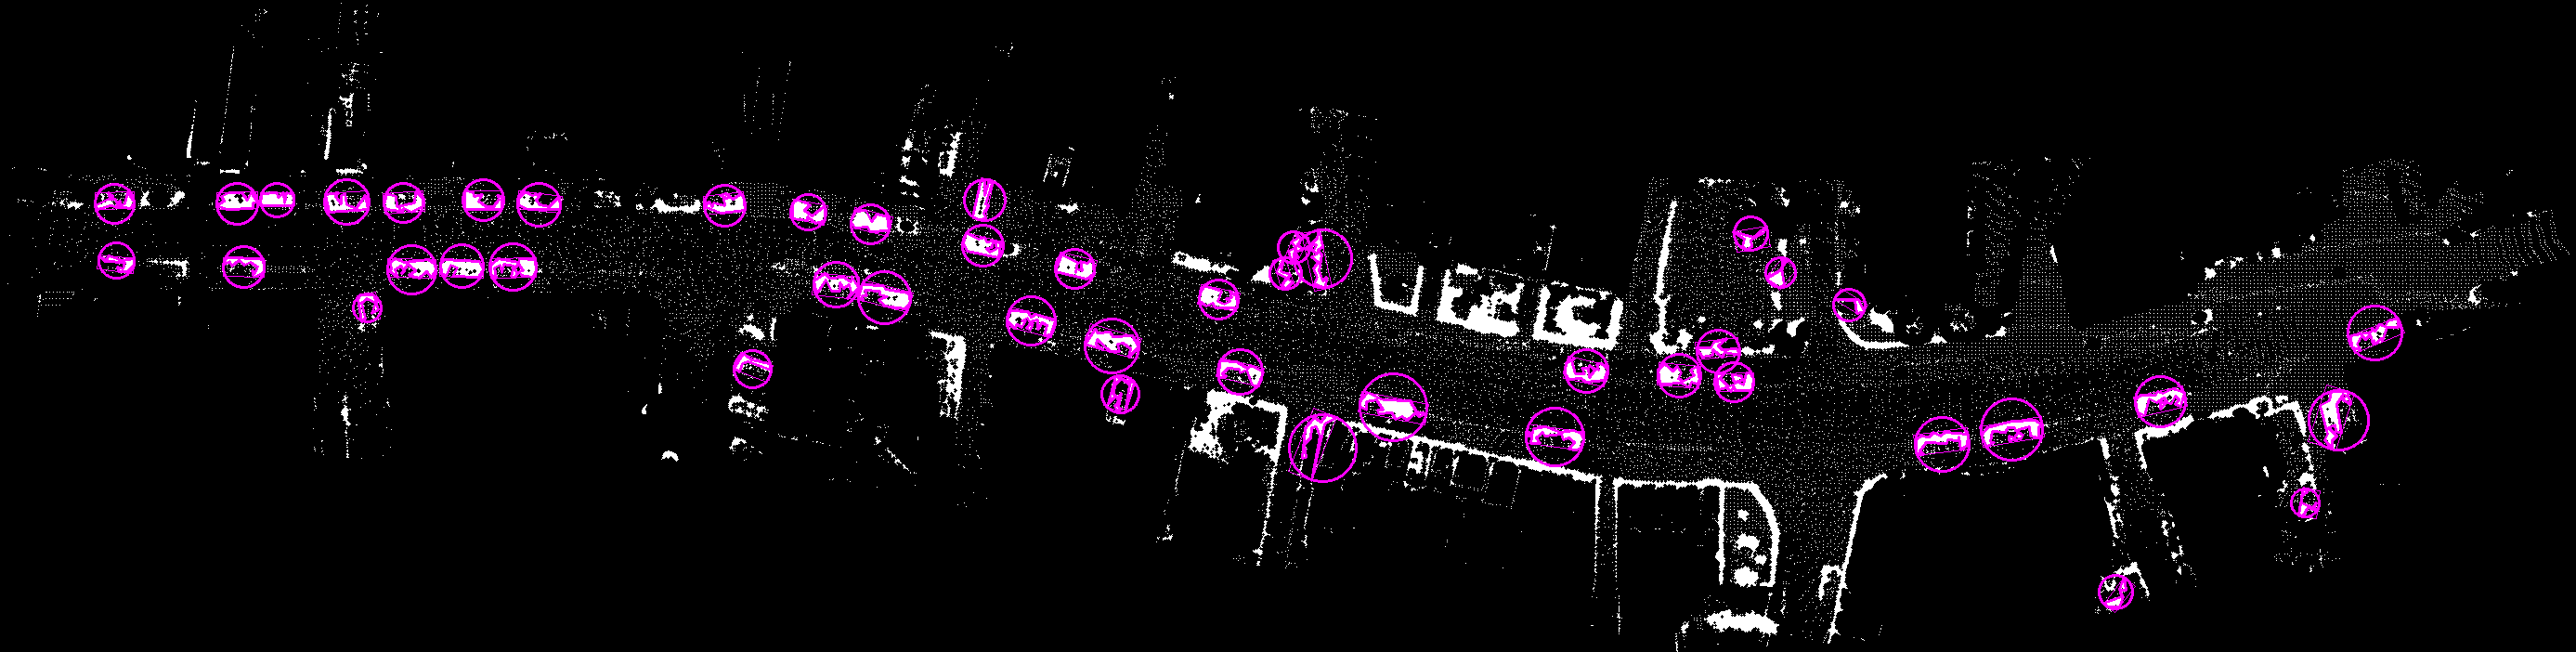
\includegraphics[width=0.92\columnwidth]{./img/ch-laser/pointsprojectedErodedWithBoundingBoxes.png}\\
    (b)
 \end{tabular}
 \caption{Car detection, $XY$ projection and processing stage}
 \label{fig:cardetection}
\end{figure}




\subsubsection{Car Detection}
In principle, we could rely on the successful multi-class image segmentation algorithms proposed, for instance, by Russel \etal \cite{russell2009associative} or by Visin \etal \cite{visin2016reseg}; however they need a learning stage which we are able to overcome exploiting the 3D data and because we look only for cars.
Few laser-based car detection algorithms have been proposed, usually they are applied in conjunction with image information and machine learning algorithms \cite{wender20083d}, \cite{zhang2014vehicle}, and \cite{premebida2007lidar}.
Here we detect cars in laser data without the need of a learning stage; the knowledge on the dimensions and shape of cars is enough to accomplish this task reliably.

First, we project the point cloud on the ground plane and we aggregate the points according to a 2D grid on the $XY$ plane similarly to what we do in the ground removal step (see Figure \ref{fig:cardetection}(a)); the cell dimension is $0.1$x$0.1$m.
Then we empty the cells containing points higher than a threshold $\tau=2.2m$ to neglect most of the walls and trees, very common in urban environments.
We treat the resulting grid as an image and we apply the closure morphological operator, to close small holes and gaps and to filter out isolated points.
We finally extract connected cells with at least one point and we keep only the regions whose bounding box has a shape compatible with a car (in red in Figure~\ref{fig:cardetection}(b)). 
Let $l_{BB}$ and $w_{BB}$ be respectively the length and width of the bounding box around a connected set of cells, and $\rho_{BB}$ the radius circumscribing the box; we filter out all the regions which do not satisfy:
\begin{equation}
 \hat{\rho}_{min} < \rho_{BB} < \hat{\rho}_{max} \quad \text{and} \quad  \hat{r}_{min} < \frac{w_{BB}}{l_{BB}}< \hat{r}_{max},
\end{equation}
where, in our case, we take into account the average dimensions of the cars and we choose $\hat{\rho}_{min} = 1.5m$, $\hat{\rho}_{max}=5.5m$,  $\hat{r}_{min} =\frac{1.2}{5.0}$ $\hat{r}_{max} = \frac{3.5}{5.0}$.

As a further filtering, we take into account the $Z$ dimension that the previous projection has neglected.
For each 2D bounding box we project the points along the direction parallel to the longest dimension between $l_{BB}$ and $w_{BB}$ (see Fig. \ref{fig:convHull}(a)) in a discrete grid, which is again composed by $0.1m$x$0.1m$ cells.
We compute the convex hull of the projected points (Fig. \ref{fig:convHull}(b)) and we treat the result as an image. 
For each column we collect the number of white pixels in a vector $\mathbf{\gamma}$; we compute the discrete derivative of $\mathbf{\gamma}$; then, we compute a three bin histogram of it as in Fig. \ref{fig:convHull}(c)).
The group of points is classified as car if the first and third bin represent respectively an increasing and a decreasing ramps of at least $\frac{\pi}{6}$ and the second bin is almost flat (at most $\frac{\pi}{3}$). 
Figure \ref{fig:drawing} shows the bounding boxes around the regions detected as cars; almost all the recognizable cars are successfully detected.
The method runs in $0.19s$ for a sequence of around $300$m, moreover even if some false negative exists, \ie, some cars are not detected, they are going to be reconstructed anyway, at least partially.


\begin{figure}[tp]
    \centering
\setlength{\tabcolsep}{1px}
    \begin{tabular}{ccc}
        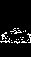
\includegraphics[width=0.3\columnwidth]{./img/ch-laser/CurProj.png}&
        
\includegraphics[width=0.3\columnwidth]{./img/ch-laser/convHull.png}&
        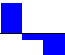
\includegraphics[width=0.3\columnwidth]{./img/ch-laser/hist}\\
        (a)&(b)&(c)
    \end{tabular}
    \caption{3D points projected on the plane parallel to the longest box dimension (a) that generate the car silhouette as convex hull (b). To classify the points we adopt an histogram representation (c)}
    \label{fig:convHull}
\end{figure}

\begin{figure}[tp]
 \centering
 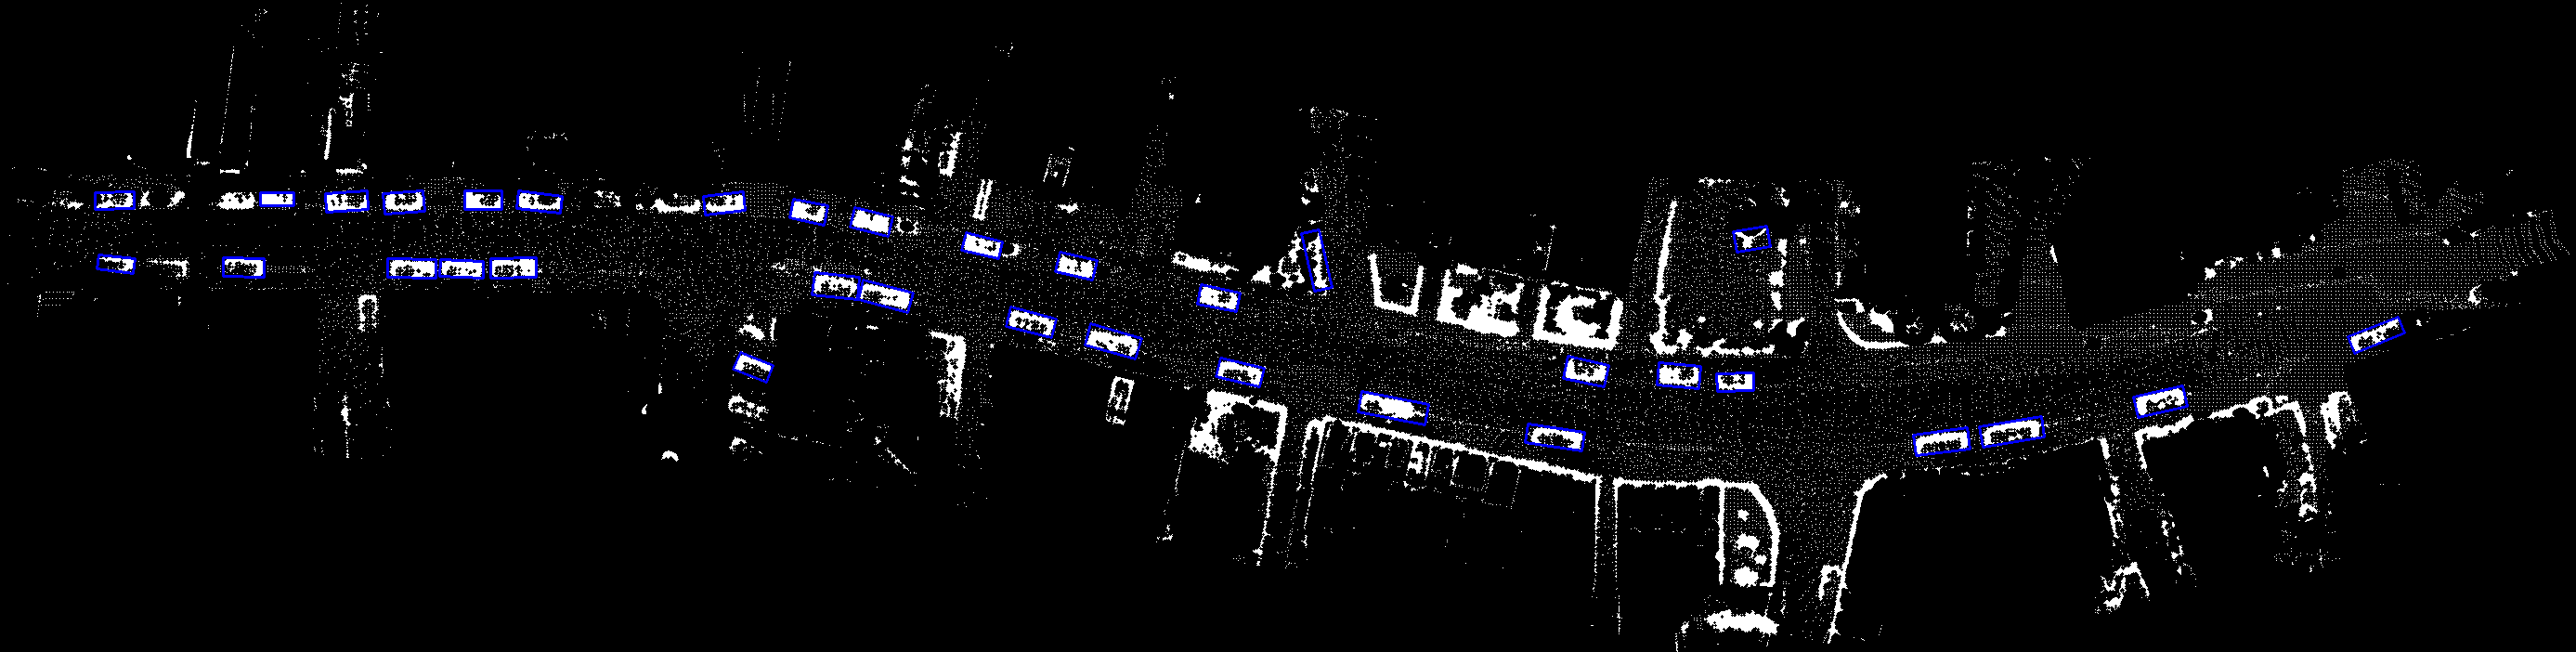
\includegraphics[width=0.98\columnwidth]{./img/ch-laser/drawing.png}
 \caption{Regions detected as cars}
 \label{fig:drawing}
\end{figure}



\subsection{Texturized reconstruction}
Once the points belonging to cars have been detected, we remove them from the point cloud of the whole scene, and we group them into a set of clusters:
\begin{equation}
Cars = \left\{c_1, \cdots, c_i, \cdots, c_{N_{cars}}  \right\},
\end{equation}
where $c_i$ represents a single cluster, \ie, a car.

To obtain a consistent reconstruction we also recover the ground points removed for the moving object detection and using the resulting point cloud, the sensor-to-point rays, and the position of the lidar in metric coordinates after each GICP registration, we are able to apply the visibility consistent mesh reconstruction algorithm presented in Chapter \ref{ch:manif}.
This is a space carving-based method which partitions the space into tetrahedra, and classifies each tetrahedron as free space or matter according to the visibility rays; the boundary between the two classes is the resulting mesh. 

%In order to reconstruct the geometry of the scene we first remove the points belonging to cars from the point cloud estimated during the moving detection stage. The moving object have been yet removed therefore we are able to apply the reconstruction algorithm proposed in \cite{romanoni15b} and \cite{romanoni15b}, where we replace the camera centers with the laser center and the visibility rays goes from laser positions to the observed 3D points.
In this context we do not need to map the environment incrementally as in \cite{romanoni15b}, especially because the texturing process has to take into account the whole set of images at the same time; therefore, we apply the batch version of the algorithm, \ie, we first add every laser center, 3D point and visibility ray, then we estimate the mesh. 

The 3D reconstruction we obtain does not contain the moving points and the cars we detected previously. 
However we aim at mapping the static part of the scene and we might consider parked cars as a part of it.
These cars have to be integrated into the final reconstruction. 
Each cluster of points $c_i \in Cars$ represents a car; and to include it into the model of the scene, we first compute its 3D convex hull then we add it to the estimated 3D map.

\subsection{Photometric Mapping and Texturized Mesh}
The removal of points belonging to cars and the explicit inclusion of their convex hull, allows a more consistent reconstruction and it overcomes the issue presented in the introduction related to the transparency of the car windows. Now, mapped cars have no more holes, and they are represented more coherently by a convex shape; of course the convex hull is not able to capture the details, but it is close enough to the real scene to allow for a photometric refinement.

At the end of the whole algorithm we aim at visualizing a textured mesh of the scene where moving objects have been removed. 
For this purpose we need to filter out the image pixels corresponding to moving objects both in the refinement and texturing processes.
We create a mask of moving objects by expanding the projection of the moving points detected previously through morphological dilation (red regions in Figure \ref{fig:mask}). 

We are now able to apply the refinement step described in \cite{vu_et_al_2012} and \cite{romanoni16}, not involving the moving parts of the scene in the optimization procedure, \ie, excluding the mask of moving objects from the refinement itself.

Eventually, we texturize the mesh with the Mask Photo Blending algorithm proposed in \cite{callieri2008masked}, where instead of taking into account all the pixels of all images to texturize the mesh, we project on the mesh only the regions of the images classified as static. 

\begin{figure}
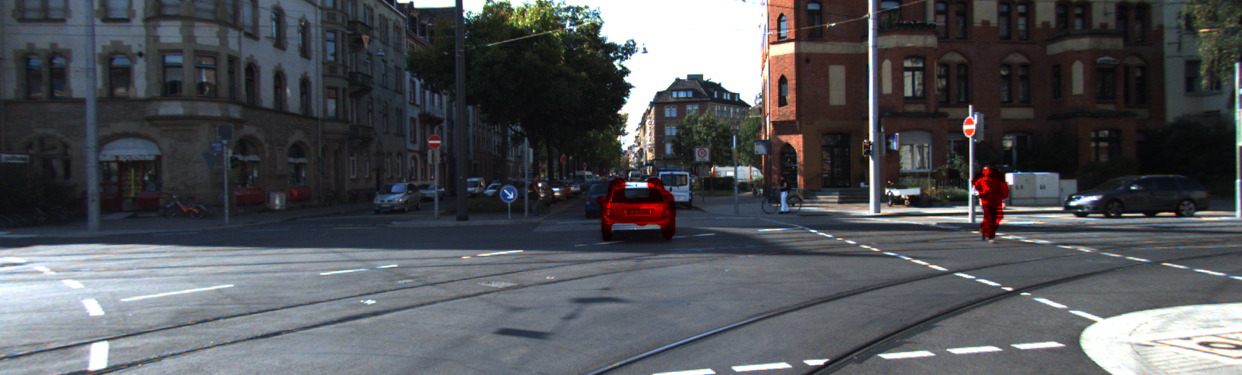
\includegraphics[width=\columnwidth]{./img/ch-laser/mask_0017}
\caption{Red regions corresponds to the moving objects}
\label{fig:mask}
\end{figure}




























% 
% In order to reconstruct the geometry of the scene we first remove the points belonging to cars from the point cloud estimated during the moving detection stage. The moving object have been yet removed therefore we are able to apply the manifold reconstruction algorithm presented in Chapter \ref{ch:manif}, where we replace the camera centers with the laser center and the visibility rays goes from laser positions to the observed 3D points.
% In this context we do not  need to map the environment incrementally, especially because the texturing process in the following takes into account the whole set of images in the same time; therefore we apply the batch version of the proposed algorithm \ie we first add every laser center, 3D point and visibility ray, then we grow the manifold.
% 
% The 3D reconstruction we obtain do not contain both the moving points and the cars we detected previously. 
% However we aim at mapping the static part of the scene and we consider parked cars as part of these. Since we looked for cars after moving points removal, all the car detected have to be integrated into the final reconstruction. 
% Each cluster of points inside a 2D bounding box estimated before, represents a car: to include it into the model of the scene, we first compute the 3D convex hull of them, then we merge the convex hull with thee algorithm described in Section \ref{sec:Mesh_merging}.
% 
% The former removal of points belonging to cars and the latter explicit inclusion of the convex hull, let the reconstruction to be more consistent and it manages to overcome the issue presented in the introduction related to the transparency of the car window. Now cars have no more holes, but they are represented more coherently by a convex shape, which of course is not able to capture the details, however is close enough for the photometric refinement.
%  
% % \cite{tanner2016lies}
% % \cite{cornelis_et_al08}
% We recall that at the end of the whole algorithm we aim at visualizing a textured mesh of the scene where moving objects have been removed. 
% For this purpose we need the image data collected together with the laser scans, but not all the image have to be used both in the texturing and in the refinement processes.
% Instead we need to project the points belonging to moving objects to each image; in order to obtain a dense region of the image, we expand the projected points through morphological dilation and we obtain a result as in Figure \textbf{FIGUREEE}. 
% 
% We now are able to texture the mesh with the Mask Photo Blending algorithm \cite{callieri2008masked}, where instead of taking into account all the pixels of the images to texturize the mesh, we project on the mesh only the regions  of the images which are not classified as moving points. 
% Analogously we are also able to apply the refinement step described in Section \ref{sec:Incremental_photoconsistent} without involving the moving part of the scene in the optimization procedure.
% 

\section{Experimental results}%%%%%%%%%%%%%%%%%%%%%%%%%%%%%%%%%%%%%%%%%%%%%%%%%%%%%%%%%%
\label{sec:experiments}
We now show experimental results on the KITTI datasets showing the effectiveness of the two main contribution described in this chapter: moving object detection and 3D reconstruction of the static part of the scene.
\subsection{Moving object detection}
To the best our knowledge a dataset with surveying camera having annotated moving objects is not available, so we tested the proposed algorithm with three sequences of KITTI \cite{Kitti} dataset, which provides 1392x512px images, camera calibration information, and Velodyne HDL-64E point clouds, where we manually annotated the moving object regions on the images. To evaluate the accuracy of the classification, we project the 3D points of each point cloud on the corresponding image plane and we check if points classified as dynamic objects project into the manually annotated masks. An example of the comparison between the resulting dynamic points and ground truth mask is shown in Figure~\ref{fig:points}.
We run the tests on a  Intel Core i7-3537u (2 Cores), 2GHz with 8GB of DDR3 RAM. 

No available code and comparison is available, therefore we compare our approach with the state-of-the-art Vallet \etal \cite{vallet2015extracting} which is the approach closer to the proposed.
In Table \ref{tab:resPR} we list the precision/recall results; our laser-based algorithm with a very small decrease of the recall, it increases significantly the precision of \cite{vallet2015extracting}, and image validation refines the results.
In Table \ref{tab:numPRobj} We show that the proposed algorithm detect or partially detect an higher number of moving object where  partially detected means that a subset of the moving points remains in the final global cloud.

In Figure~\ref{fig:roc} we report the Receiver Operating Characteristics (ROC) curve obtained with the 0095 sequence: here we compare the ground truth mask against an image-based mask of moving objects obtained b a simple dilation of the points classified as moving and projected in the image plane, to have a resutl similar to background subtraction algorithms. 
The ROC curve the highest the area subtended by the curve, the better the performance; precision and recall reported in the plot are obtained by varying the $\sigma_r$ and $\sigma_{\theta}$ parameters such that $0.1m<\sigma_r<0.45m$ and $0.0035rad<\sigma_{\theta}<0.0088rad$.
The results enforce the conclusion that the proposed approach performs better that the algorithm by Vallet \etal already in the lidar-based only version and shows the overall improvement with the image-based validation. Indeed, the discretization and diffusion of occupancy information lead to smoother and more precise results.

Our algorithm outperforms the work by Vallet \etal also in terms of computing speed, thanks to the use of octree indexing and subsampling. 
Indeed, our algorithm takes around 0.6 seconds per point cloud, while Vallet \etal approach takes 4.9 seconds.
Timing does not include the image-based validation step: it has been implemented as a prototype in MATLAB and at the current stage it works off-line at 25 seconds per frame to estimate the depth map and 1-2 seconds to validate the moving points; nevertheless, this step can be easily parallelized on GPU leading to real time computations.

The ROC curves also show that both the novel laser-based pipeline and the image validation procedure improve significantly the precision of the proposed algorithm, in particular the validation has been able to discard a huge number of false positive in moving objects detection.

% \begin{figure}[t]
% \centering
% 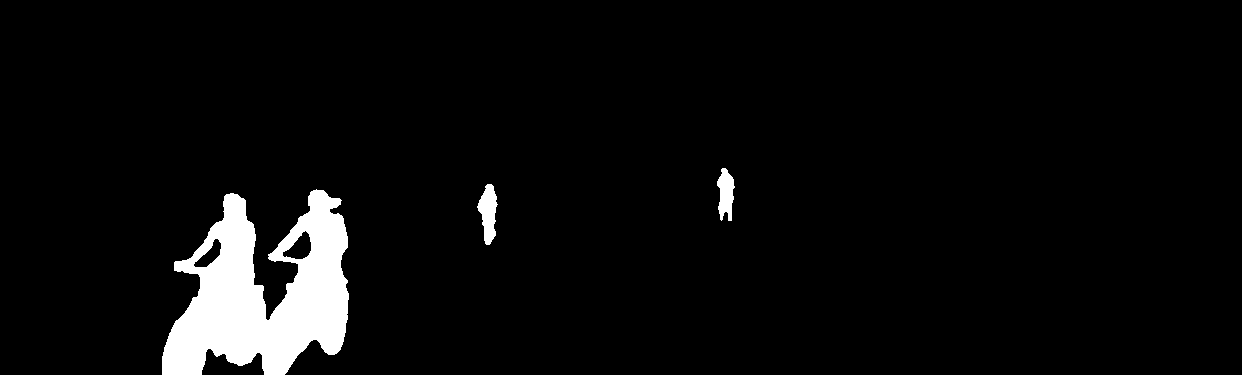
\includegraphics[width=0.98\columnwidth]{mask-129}
% \caption{Ground-truth moving objects mask.}
% \label{fig:gt}
% \end{figure}
% \begin{figure}[t]
% \centering
% 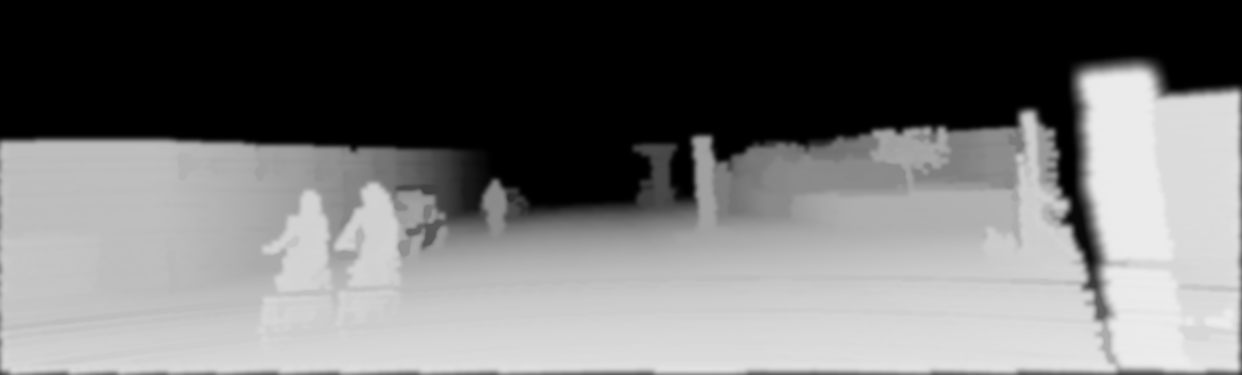
\includegraphics[width=0.8\columnwidth]{./img/ch-laser/depth-0129}
% \caption{Example of a depthmap computed from a lidar point cloud.}
% \label{fig:depth-map}
% \end{figure}

\begin{figure}[t]
\centering
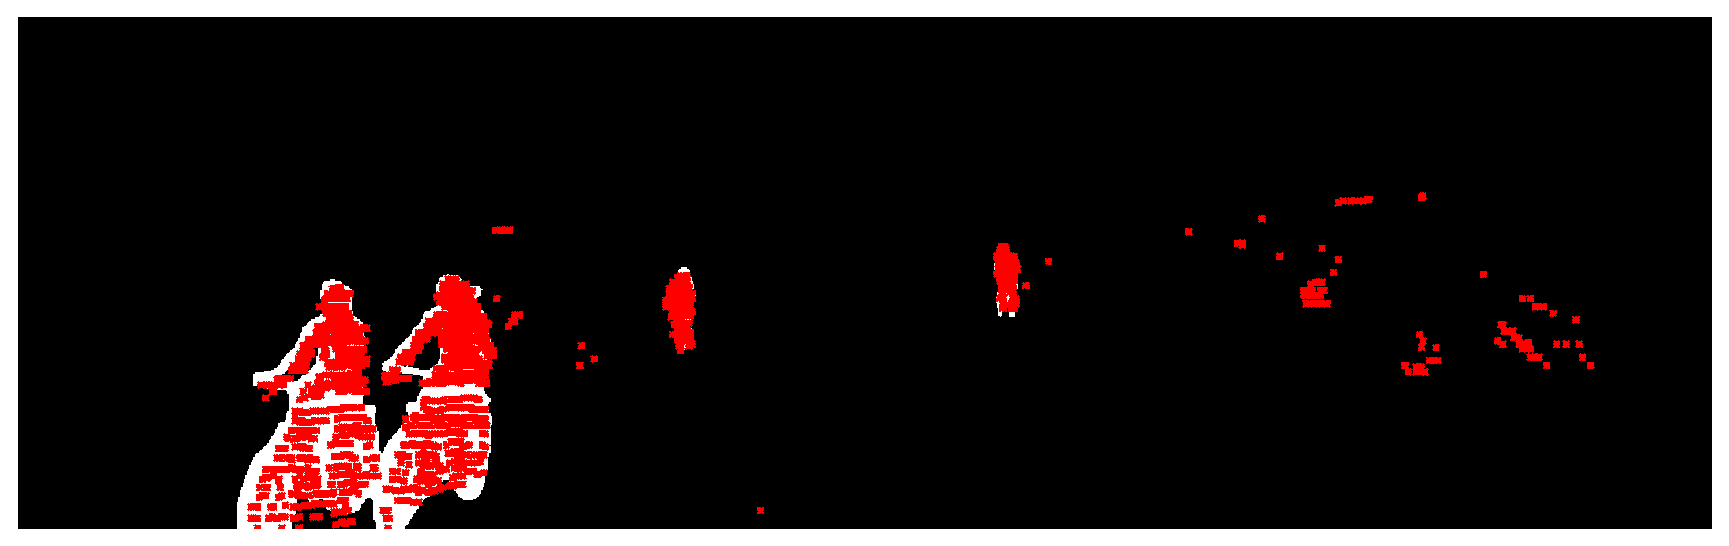
\includegraphics[width=0.98\columnwidth]{./img/ch-laser/points_result_on_mask}
\caption{Points classified as moving projected against the ground-truth mask.} 
\label{fig:points}
\end{figure}




\begin{table}[t]
\caption{Precision/recall results on KITTI sequences.}
\label{tab:resPR}
\centering
\setlength{\tabcolsep}{3px}
\begin{tabular}{lcccccc}
\toprule                                                                                
&\multicolumn{2}{c}{seq 0091}&\multicolumn{2}{c}{seq 0095}&\multicolumn{2}{c}{seq 0104}\\
&P & R &P & R &P & R \\
\midrule
Vallet el al. \cite{vallet2015extracting}       &       0.11&\textbf{0.80}      &       0.10&\textbf{0.81}      & 0.27&\textbf{0.90}\\
proposed laser-based                            &   0.25&0.75   &  0.19&0.79    & 0.44&0.87\\
proposed w/ image validation                            &       \textbf{0.26}&0.73      &  \textbf{0.24}&0.76   & \textbf{0.49}&0.89\\
\end{tabular}
\end{table}


\begin{table}[t]
\caption{Number of  moving objects Detected (D) and partially detected (PD).}
\label{tab:numPRobj}
\centering
\begin{tabular}{lcccccc}
\toprule 
&\multicolumn{2}{c}{seq 0091}&\multicolumn{2}{c}{seq 0095}&\multicolumn{2}{c}{seq 0104}\\
&D & PD &D & PD &D & PD \\
\midrule
Vallet el al. \cite{vallet2015extracting}       & 6/20  & 7/20  & 8/8 &   0/8   &    1/6        & 3/6\\
proposed & \textbf{8/20}        & \textbf{9/20} & 8/8 &   0/8   &    \textbf{3/6}       & 3/6 \\
\end{tabular}
\end{table}

\begin{figure}[t]
\centering
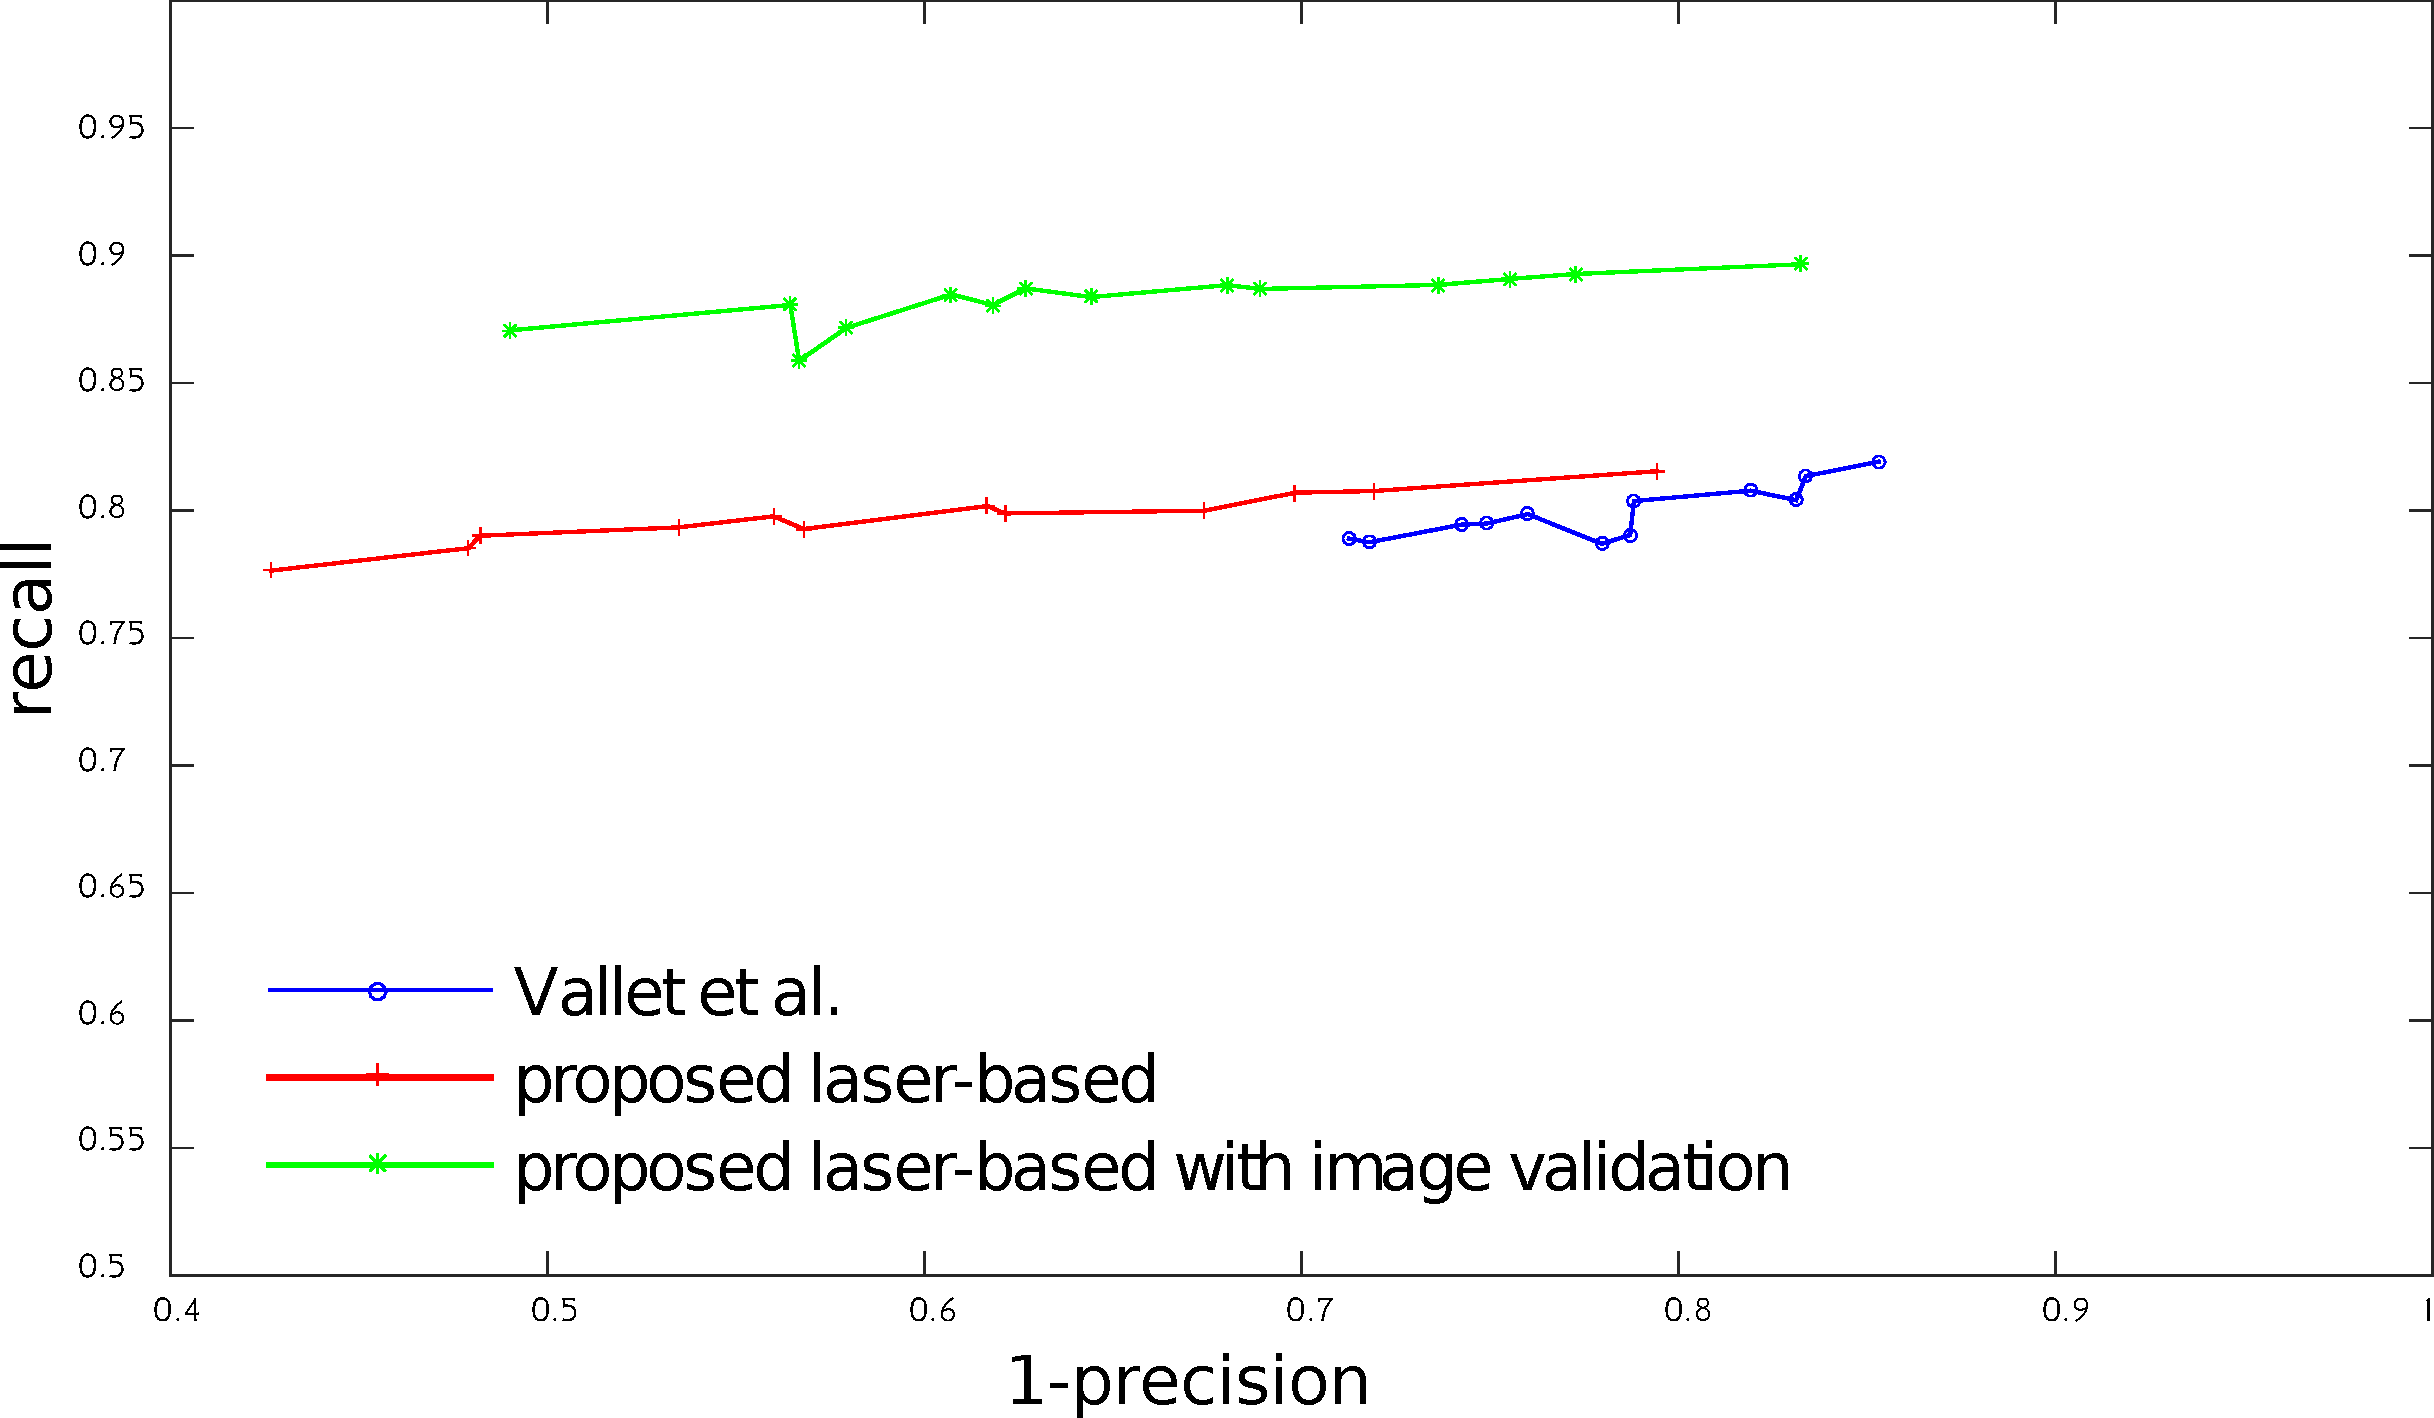
\includegraphics[width=0.98\columnwidth]{./img/ch-laser/graphres3}
\caption{ROC of  \cite{vallet2015extracting} and our algorithms.}
\label{fig:roc}
\end{figure}

\subsection{3D Reconstruction}
% We tested the refinement and texturing our approach against the publicly available KITTI dataset \cite{geiger_et_al12}; in particular we used the sequences 0095 and 0104, captured by a Velodyne 64HD with respectively 268 and 313 1392x512 gray scale frames. 
% The algorithm runs on a 4 Core i7-920 CPU at 2.6Ghz (8M Cache), with 24GB of DDR3 SDRAM endowed with a NVIDIA TitanX.

In order to provide a quantitative evaluation of the refinement and texturing, we compare the reconstructed meshes against the full point cloud, \ie, without the downsampling needed for moving object detection (see Section~ \ref{sec:ground_removal}). Lidar data are dense and accurate enough to be considered as ground truth. 
We removed from the full point cloud both the moving point and the interior of the cars we do not want to map.
The mesh to point cloud comparison was computed by the tool CloudCompare \cite{cloudcompare} which averages the distances from each point of the ground truth, to the  nearest triangle in the estimated mesh.

We compare our algorithm against different approaches applied to the same downsampled point cloud to provide a fair evaluation: the method proposed in the Chapter \ref{ch:manif} without refinement and car detection; two widespread algorithms for mesh reconstruction from point clouds, \ie, Poisson Reconstruction \cite{kazhdan2006poisson} and Ball Pivoting \cite{bernardini1999ball}; and OctoMap \cite{hornung2013octomap}, \ie, state-of-the-art laser-based mapping algorithms.

In Table~\ref{tab:res} we show the result of our comparison  the method of Chapter \ref{ch:manif}.
The average errors are below 0.1 m which is enough accurate for a wide variety of robotics tasks, such as localization and navigation. 
The proposed algorithm improves the accuracy of the basline algorithm directly applied to laser data; both car detection and photometric refinement have contributed to this enhancement. 
Since the number of cars in the 0104 sequence is greater than those in sequence 0095, the improvement is more evident in the former case.

Poisson Reconstruction was not able to produce a proper reconstruction due to the sparsity of the downsampled laser data; for the same reason Ball Pivoting produces big holes in the reconstruction and Octomap was not able to recover a dense structure. 
In addition to holes, Ball Pivoting reconstructs a mesh whose normals are not consistent and contains severe self intersections (see Fig. \ref{fig:ball}).
Moreover, while the appearance of the results of the proposed algorithm, of the baseline algorithm and, to some extent, of the Ball Pivoting are realistic, Octomap reconstructs a voxelized map in which many details are lost (see  Fig.~\ref{fig:resultOcto01}).

The algorithm reconstructed and refined the 0095 (268 frames) sequence in 73 minutes and the sequence 0104 (313 frames) in 80 minutes.

%In Table \ref{tab:dimension} we show that even if our approach is able to capture finer details of the scene, the resulting map is smaller than the map produced by octomap 
%Even if Octomap aims at representing the scene in a compact map, the approach both \cite{romanoni15b} and the proposed approach result in a smaller map.
%confronto tempi e 

\begin{table}[t]
\caption{Results on KITTI sequences: map error}
\label{tab:res}
\centering
\setlength{\tabcolsep}{3px}
\begin{tabular}{lcccc}
\toprule           
&\multicolumn{2}{c}{seq 0095}&\multicolumn{2}{c}{seq 0104}\\
&avg & std  &avg & std \\
\midrule
baseline & 0.089&0.131 & 0.194 & 0.311\\
after car detection  & 0.085&0.099 & 0.087 & 0.123\\
after refinement  & \textbf{0.082}&\textbf{0.098} &  \textbf{0.082}&\textbf{0.103} \\
\end{tabular}
\end{table}


% \begin{table}[t]
% \caption{Dimension of map reconstructed.}
% \label{tab:dimension}
% \centering
% %\setlength{\tabcolsep}{3px}
% \begin{tabular}{lcc}
% \toprule           
% &seq 0095&seq 0104\\
% \midrule
% \cite{hornung2013octomap} & 250 MB&   \\
% \cite{romanoni15b} & 18 MB & 8 MB \\
% Proposed approach  & 28 MB  & 31 MB\\
% \end{tabular}
% \end{table}


\begin{figure}[tp]
 \centering
\setlength{\tabcolsep}{2px}
    \begin{tabular}{c}
    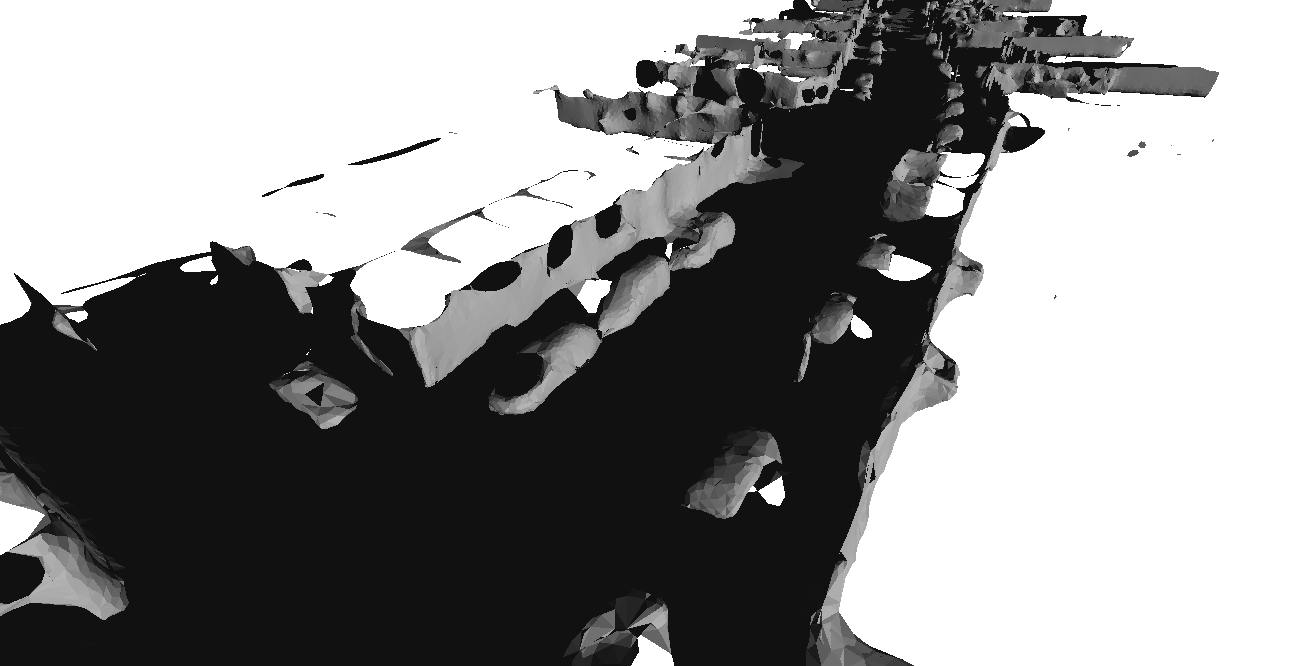
\includegraphics[width=0.98\columnwidth]{./img/ch-laser/ball00}\\
    \end{tabular}
 \caption{Ball Pivoting reconstruction: dark regions are caused by non consistent facet normals}
 \label{fig:ball}
\end{figure}

\begin{figure}[tp]
 \centering
\setlength{\tabcolsep}{2px}
    \begin{tabular}{cc}
    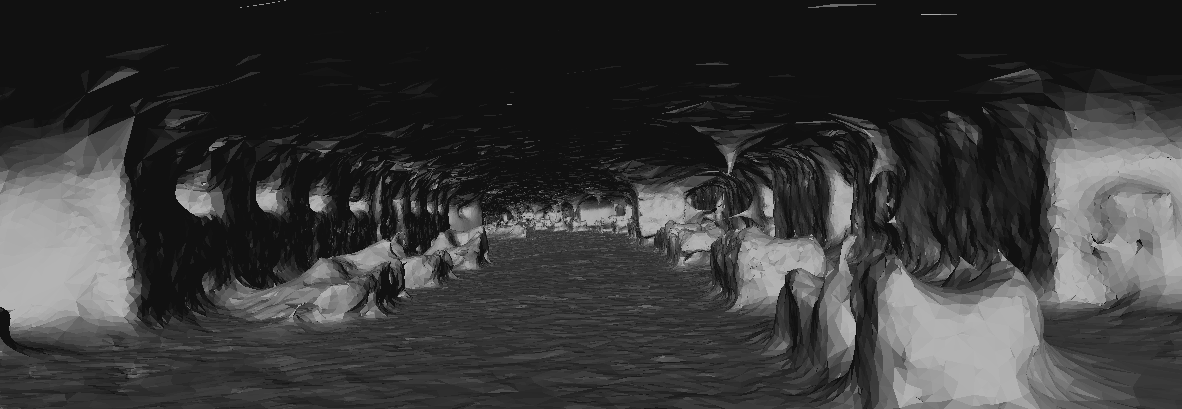
\includegraphics[width=0.45\columnwidth]{./img/ch-laser/notCar01}&
    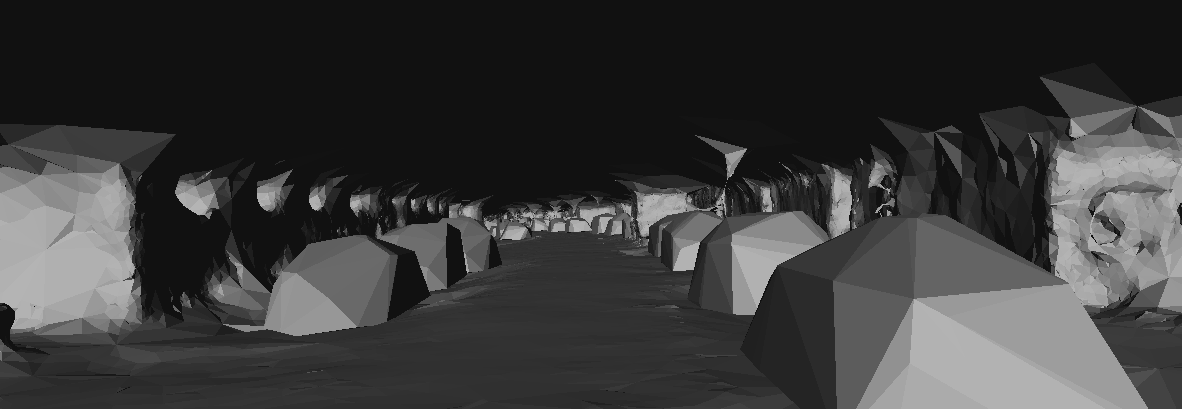
\includegraphics[width=0.45\columnwidth]{./img/ch-laser/onlyCar01}\\
    (a) Without cars detection&
    (c) With cars convex hulls\\
    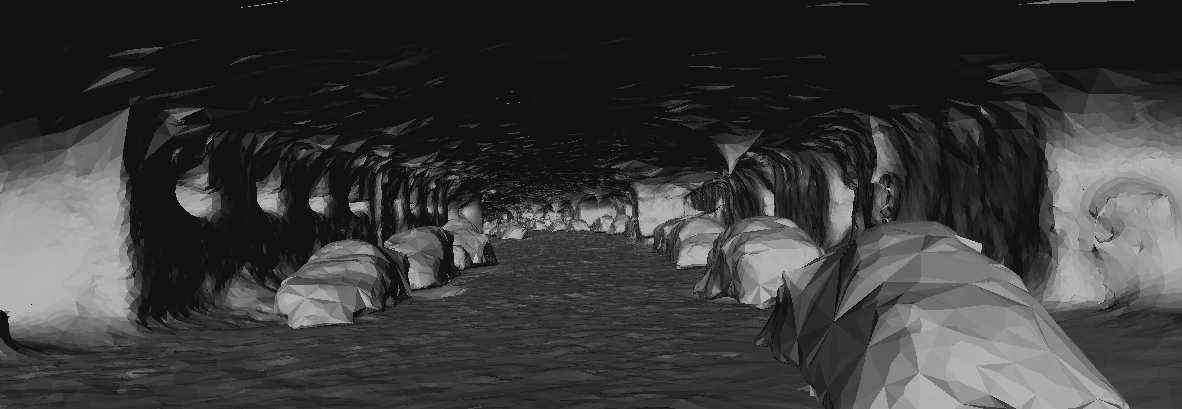
\includegraphics[width=0.45\columnwidth]{./img/ch-laser/nottextured01}&
    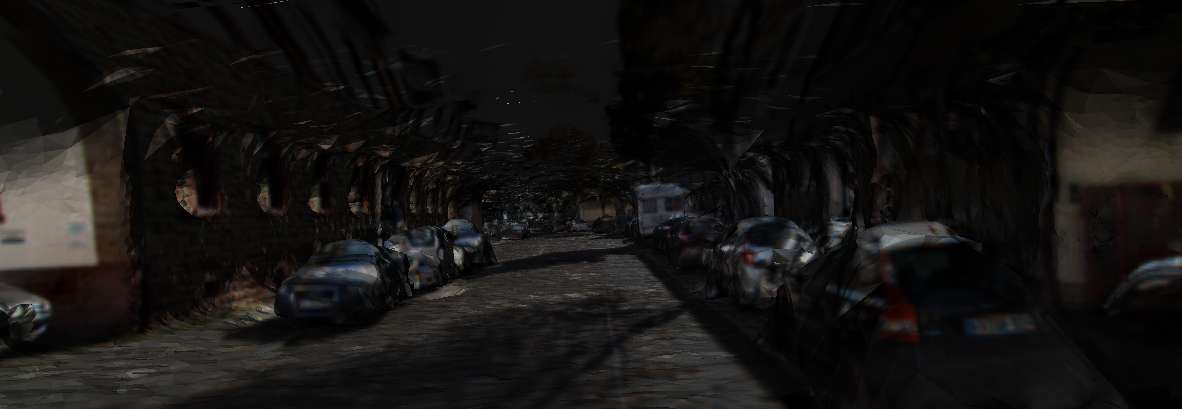
\includegraphics[width=0.45\columnwidth]{./img/ch-laser/textured01}\\
    (d) After refinement&
    (d) Refinement and texturing\\
    \multicolumn{2}{c}{
    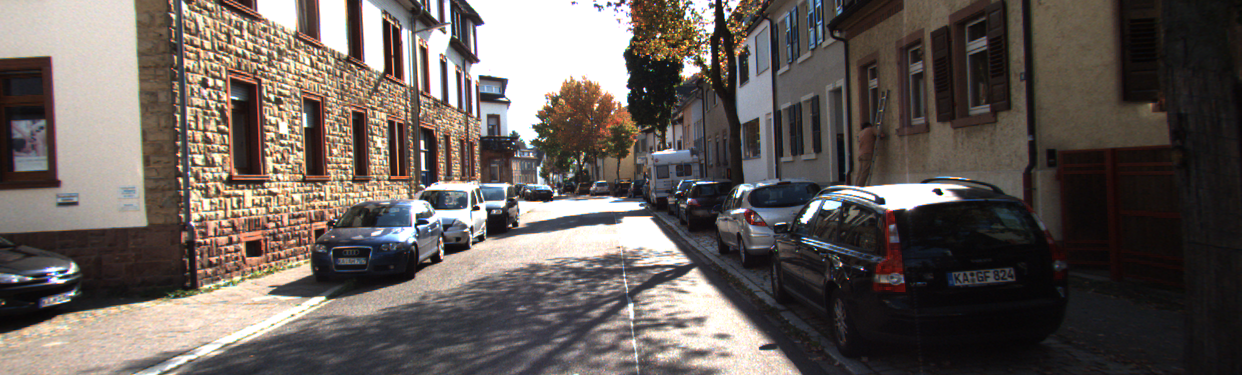
\includegraphics[width=0.92\columnwidth]{./img/ch-laser/0000000016}}\\
    \multicolumn{2}{c}{(e) corresponding frame}
 \end{tabular}
 \caption{Results on frame 16. Let notice that moving objects (the people by bicycle) do not affect the reconstruction}
 \label{fig:results06}
\end{figure}


% \begin{figure}[tp]
%  \centering
% \setlength{\tabcolsep}{2px}
%     \begin{tabular}{cc}
%   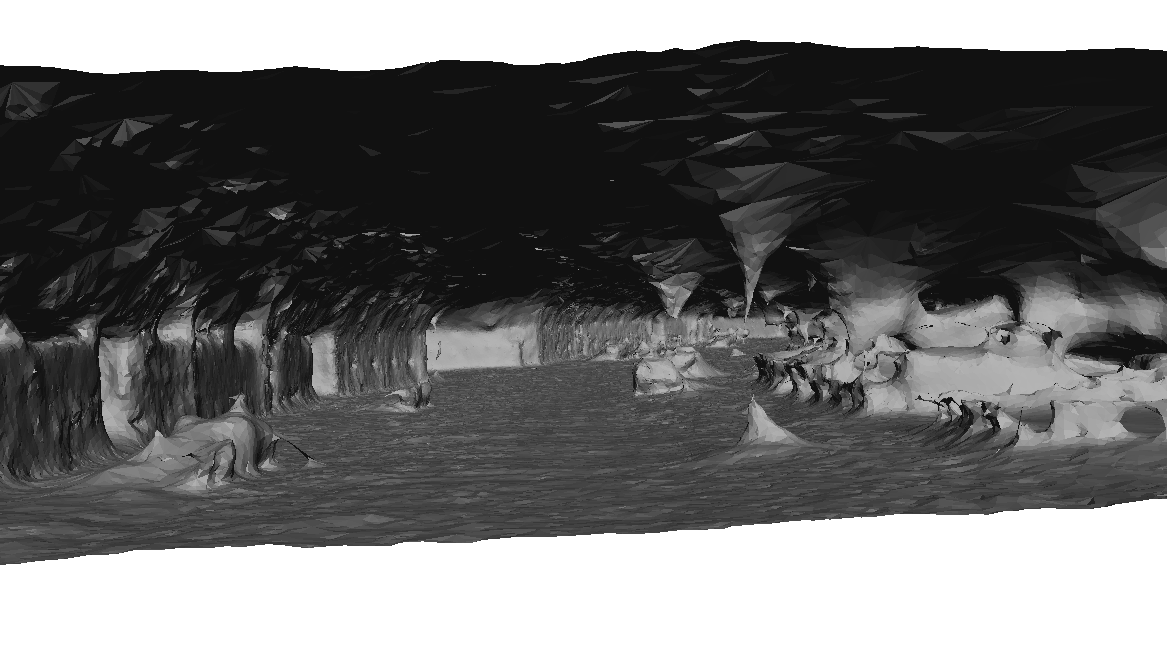
\includegraphics[width=0.24\columnwidth]{notCar00}&
%   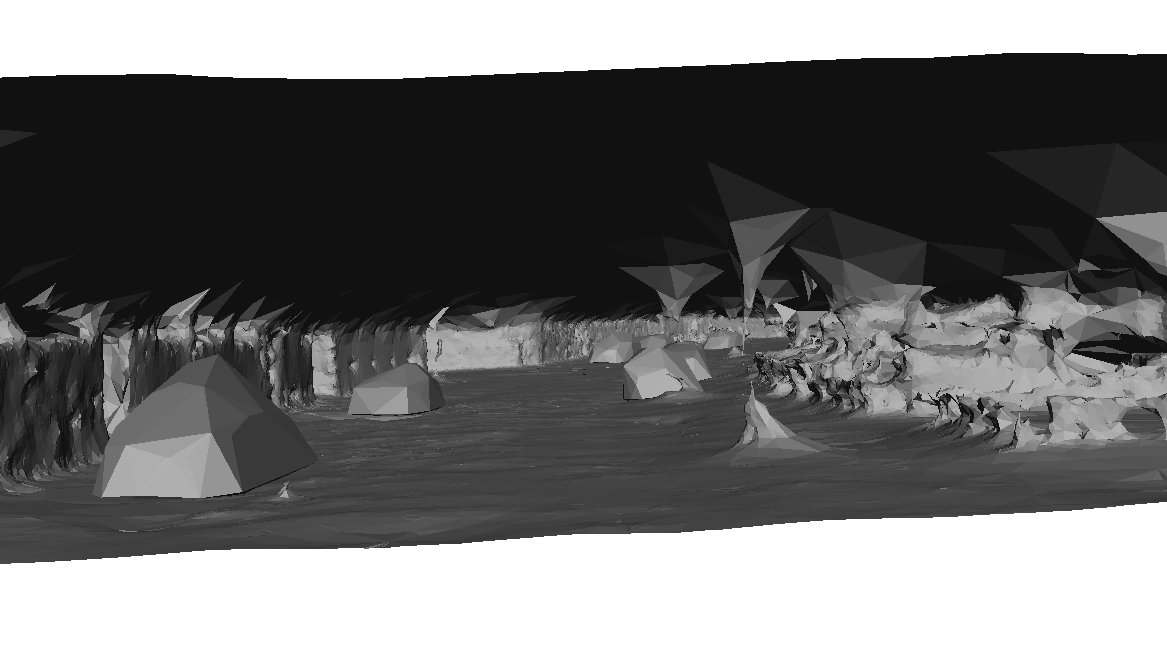
\includegraphics[width=0.24\columnwidth]{car00}\\
%   (a) Without cars detection&
%     (c) With cars convex hulls\\
%   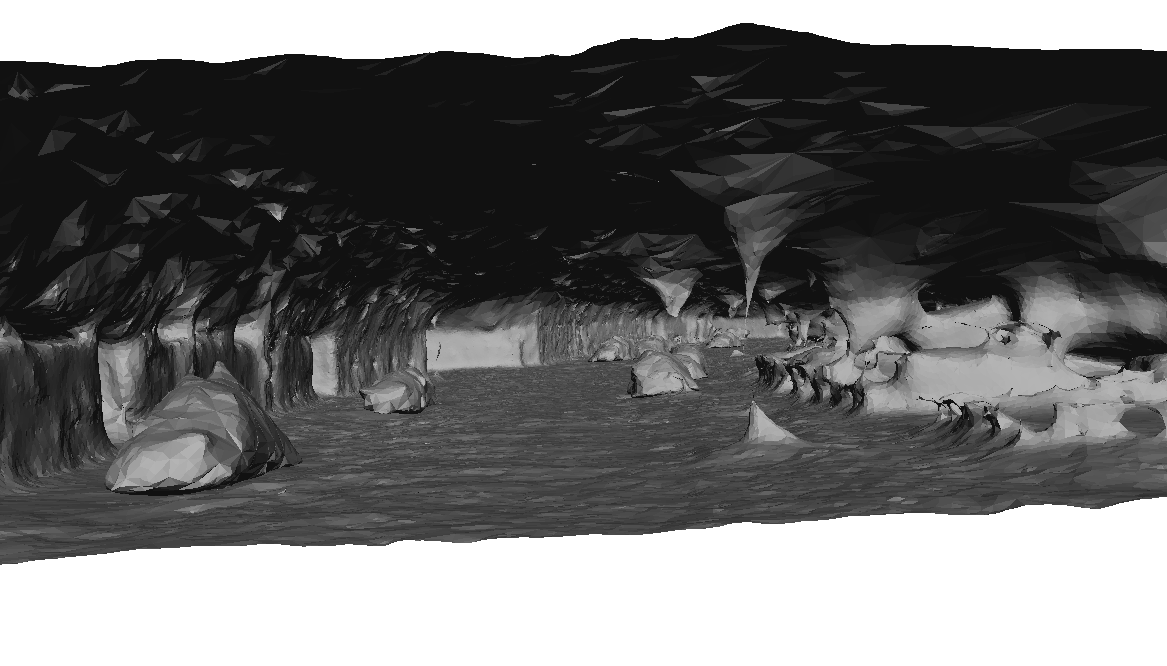
\includegraphics[width=0.24\columnwidth]{nottextured00}&
%   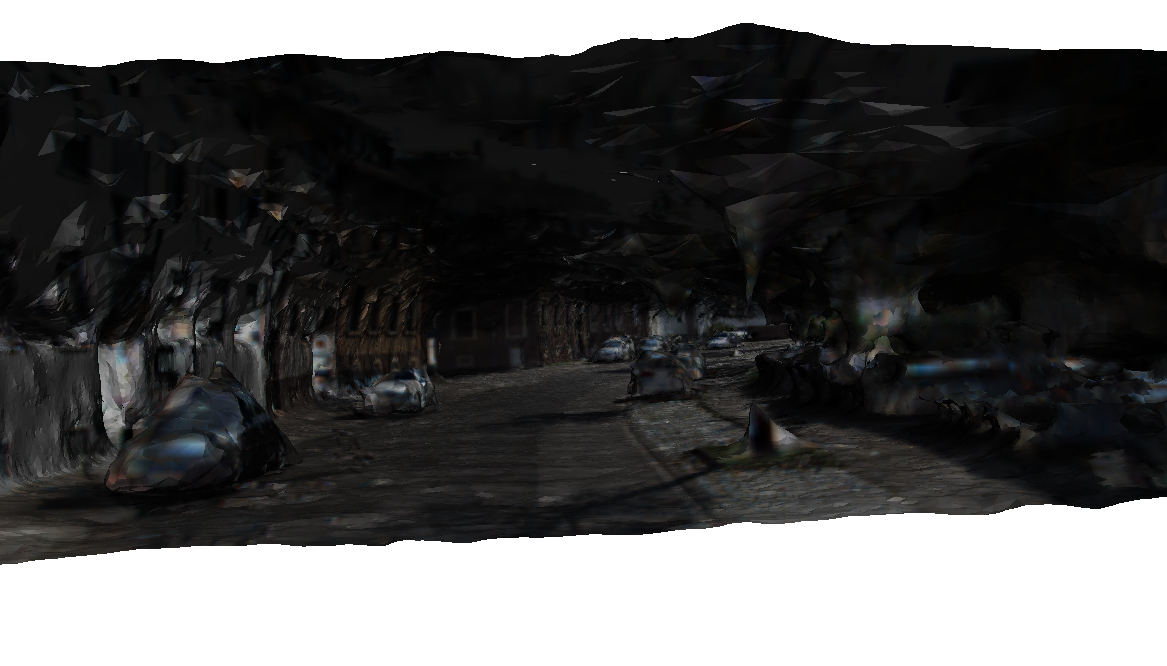
\includegraphics[width=0.24\columnwidth]{textured00}\\
%     (d) After refinement&
%     (d) Refinement and texturing\\
%     \multicolumn{2}{c}{
%   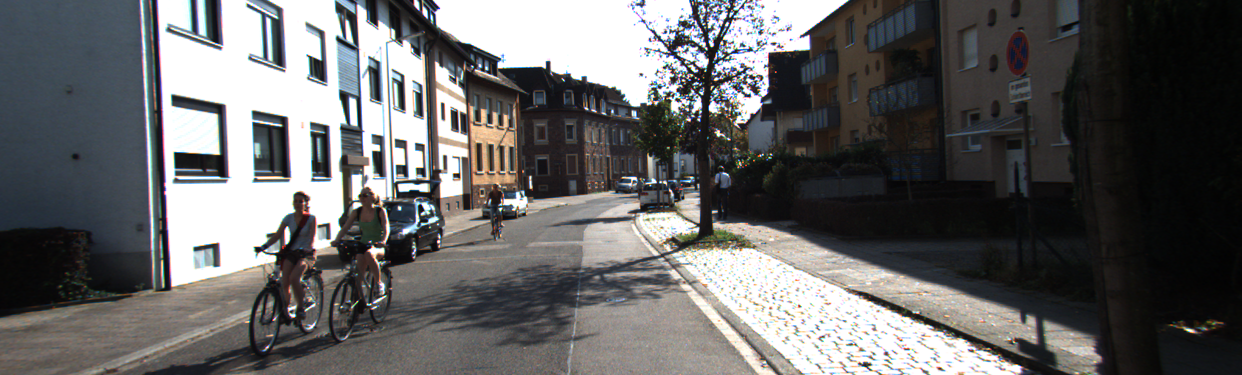
\includegraphics[width=0.48\columnwidth]{0000000128}}\\
%     \multicolumn{2}{c}{(e) corresponding frame}
%  \end{tabular}
%  \caption{Results on frame 128. Let notice that moving objects (the people by bicycle) do not affect the reconstruction}
%  \label{fig:results}
% \end{figure}


\begin{figure*}[tb]
 \centering
\setlength{\tabcolsep}{1px}
    \begin{tabular}{cc}
    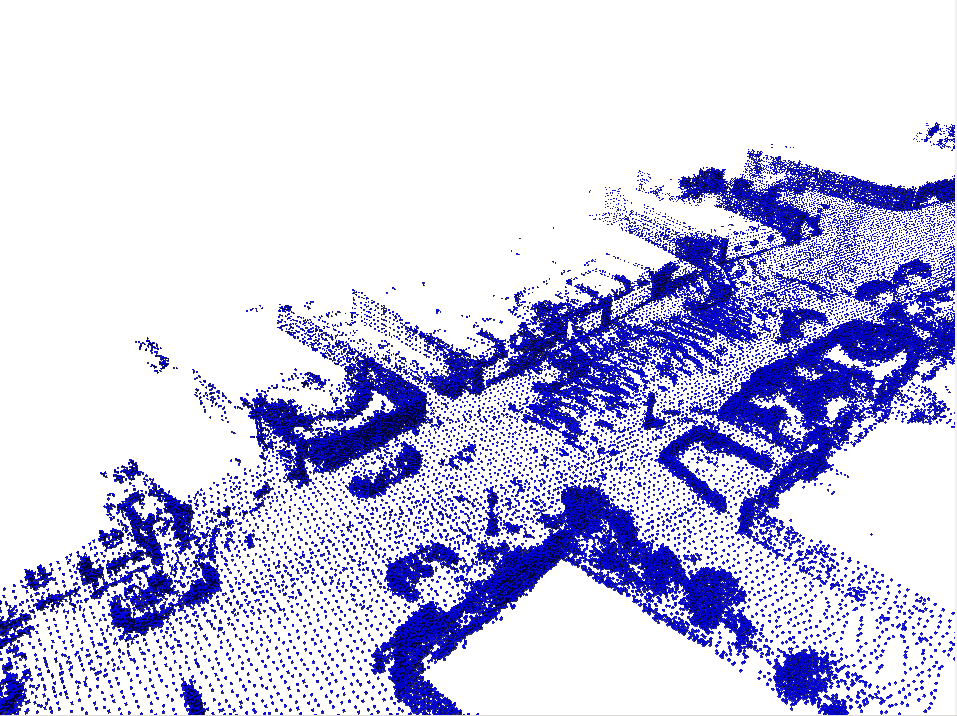
\includegraphics[width=0.45\columnwidth]{./img/ch-laser/octo06}&
    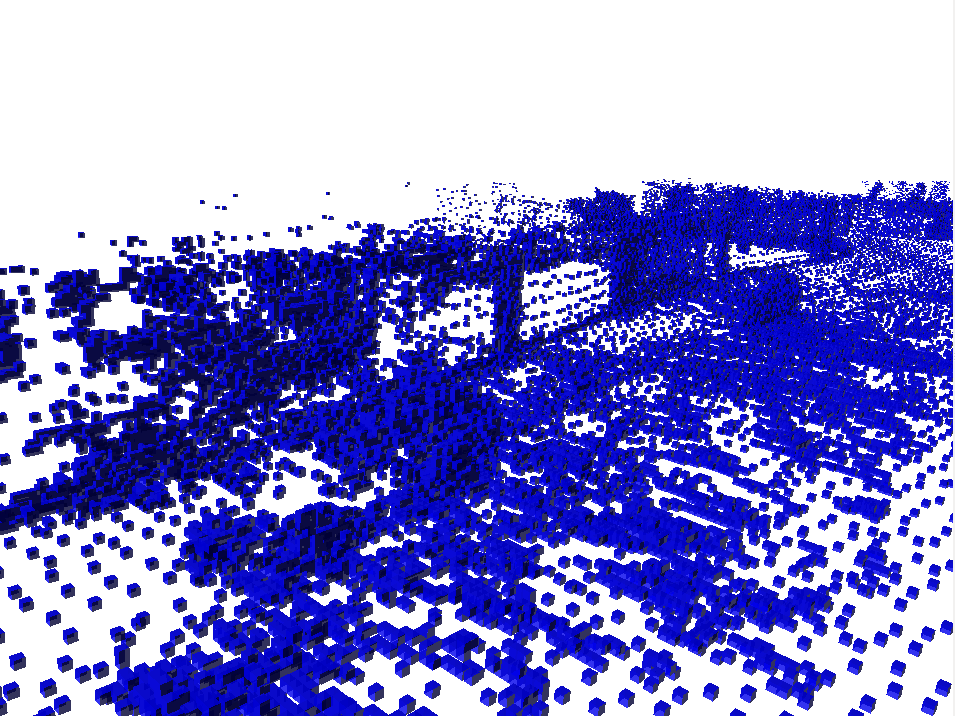
\includegraphics[width=0.45\columnwidth]{./img/ch-laser/octo05}\\
    \multicolumn{2}{c}{Octomap}\\
    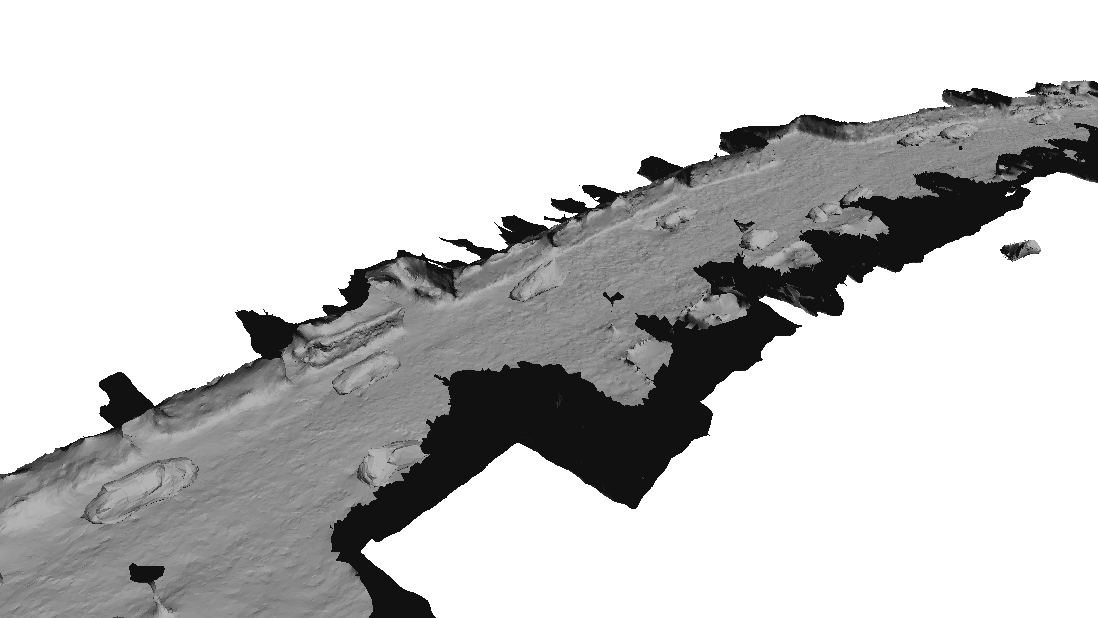
\includegraphics[width=0.45\columnwidth]{./img/ch-laser/proposed0600}&
    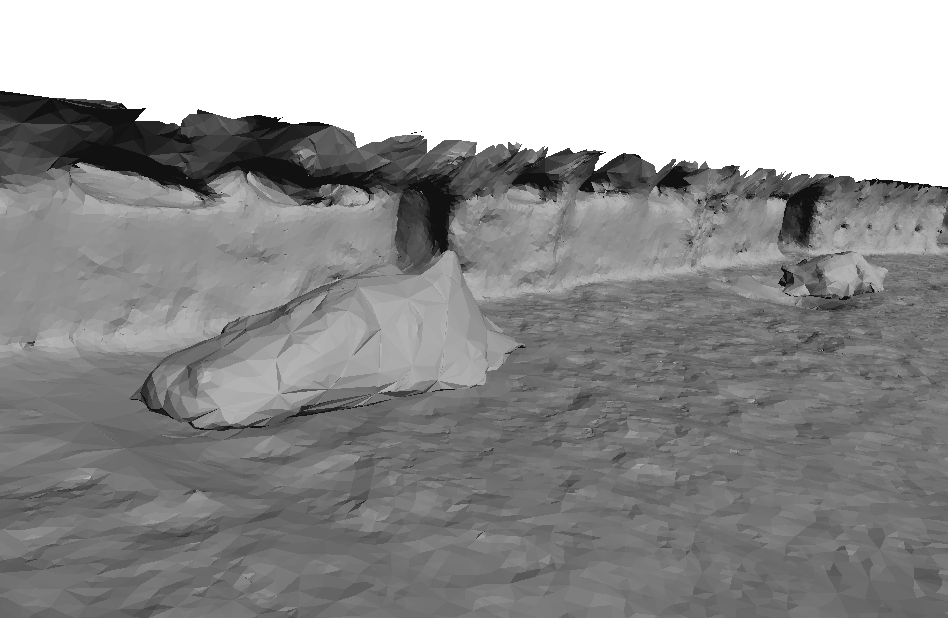
\includegraphics[width=0.45\columnwidth]{./img/ch-laser/proposed0501}\\
    \multicolumn{2}{c}{Proposed}\\
    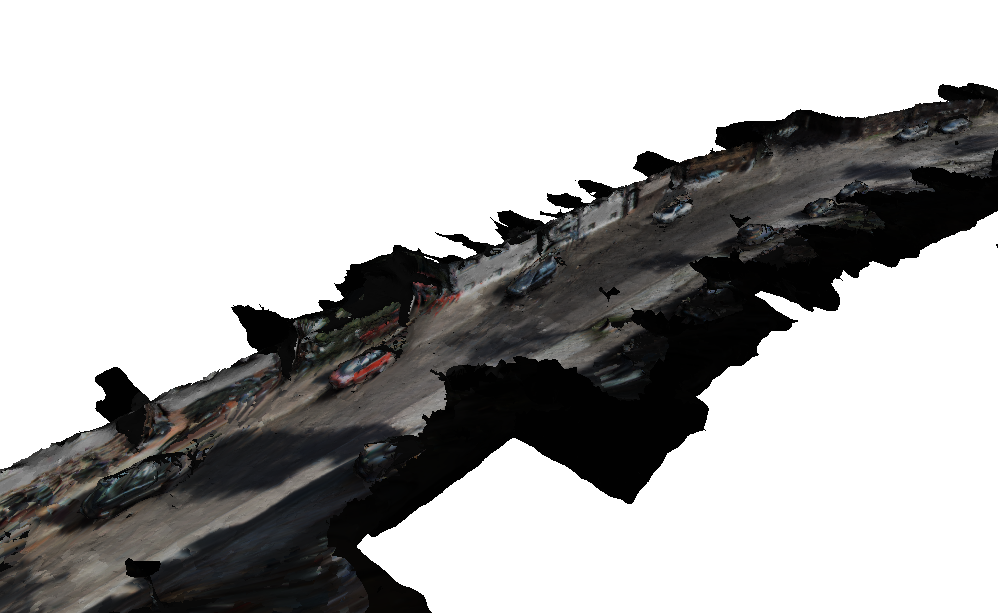
\includegraphics[width=0.45\columnwidth]{./img/ch-laser/proposed0601}&
    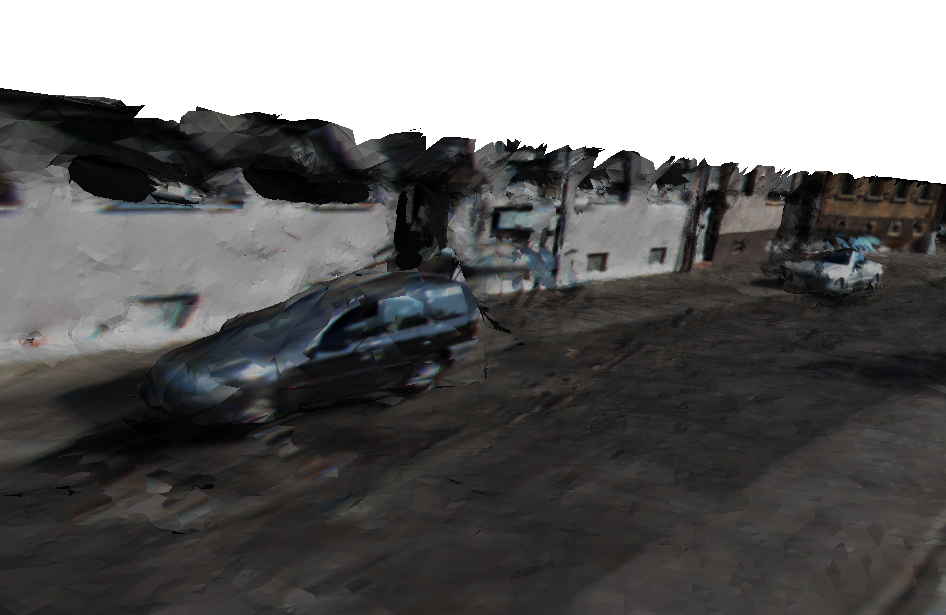
\includegraphics[width=0.45\columnwidth]{./img/ch-laser/proposed0500}\\
    \multicolumn{2}{c}{Proposed(textured)}\\
 \end{tabular}
 \caption{Reconstruction of 0095 sequence with Octomap and the proposed approach: first column whole sequence, second column detail}
 \label{fig:resultOcto01}
\end{figure*}



